\documentclass[11pt]{article}

\usepackage[margin=1in]{geometry}
\usepackage{amsmath,amssymb,amsthm,bm,mathtools}
\usepackage{booktabs}
\usepackage{graphicx}
\usepackage{microtype}
\usepackage{siunitx}
\usepackage{xcolor}
\usepackage{hyperref}
\usepackage[nameinlink,noabbrev]{cleveref}

\hypersetup{colorlinks=true,linkcolor=blue!45!black,
  citecolor=blue!45!black,urlcolor=blue!45!black}

\newcommand{\R}{\mathbb{R}}
\newcommand{\T}{\mathbb{T}}
\newcommand{\G}{\mathcal{G}}
\newcommand{\Gtheta}{\mathcal{G}_{\theta}}
\newcommand{\D}{\mathrm{D}}
\newcommand{\dd}{\,\mathrm{d}}
\newcommand{\ip}[2]{\left\langle #1,#2\right\rangle}
\newcommand{\norm}[1]{\left\lVert #1\right\rVert}
\newcommand{\project}{P_K}

\title{A Structure-Constrained Neural Surrogate for the\\
Dirichlet--Neumann Operator in Nonlinear Water-Wave Simulation}
\author{Jonathan Ma}
\date{Draft of \today}

\begin{document}
\maketitle

\begin{abstract}
We study neural approximation of the finite-depth Dirichlet--Neumann operator
for the two-dimensional irrotational water-wave problem with one horizontal
coordinate.
The central difficulty is that a small error in one operator evaluation need
not remain small after repeated use inside a Hamiltonian time integrator.  Our
surrogate retains the exact zeroth- and first-order Craig--Sulem terms and
represents only the second- and higher-order contribution by a self-adjoint
neural residual.  Its training objective combines relative $L^2$ data
misfit with Fourier-mode, local translation-tangent, and Hadamard
shape-derivative consistency terms.  Reference trajectories use a
double-precision order-six Craig--Sulem expansion, padded nonlinear products,
and an integrating-factor two-stage Gauss--Legendre method.  The reported
checkpoints use the historical v9 snapshot archive.  The parameterized,
case-split replacement dataset specified in this paper is complete and
source-authenticated, but no reported checkpoint was trained on it.

An unguarded 320-trajectory test of an earlier model with the same structural
decomposition contains no nonfinite surrogate rollout, although two finite
Tanaka trajectories exceed unit relative surface error.  Under the stated
soliton-selective guarded protocol, the selected model remains finite in all
320 registered rollouts drawn from ten panels representing five initial-wave
families.  Among the 305 cases with valid reference trajectories, the terminal
relative surface error has median $0.00285$ and 95th percentile $0.04769$.
Removing only the Fourier-mode term improves one-step validation error but
worsens the pooled terminal 95th percentile by $31\%$ and the mean by $45\%$.
These results show that one-step value accuracy alone does not predict the
long-time error tail.  They also leave a clear limitation: the strongest
current accuracy result is conditional on the declared guard, and its worst
remaining error is a finite Tanaka error.
\end{abstract}

\section{Problem introduction}
\label{sec:introduction}

We consider two-dimensional, inviscid, incompressible, irrotational gravity
waves over a horizontal bed. The free surface is represented by
$y=\eta(x,t)$, the undisturbed depth is $h>0$, and
$\xi(x,t)=\phi(x,\eta(x,t),t)$ is the trace of the velocity potential on the
free surface. Gravity acts with acceleration $g>0$. The horizontal coordinate
is periodic, $x\in\T_L=\R/(L\mathbb Z)$, with period \(L>0\). The potential
solves
\begin{align}
  \Delta\phi &= 0 && -h<y<\eta(x,t), \\
  \partial_y\phi &= 0 && y=-h, \\
  \phi &= \xi && y=\eta(x,t).
\end{align}
The Dirichlet--Neumann operator (DNO) maps the surface potential to the
unnormalized upward normal derivative,
\begin{equation}
  \G(\eta;h)\xi
  =\left(\partial_y\phi-\eta_x\partial_x\phi\right)_{y=\eta(x,t)}.
  \label{eq:dno-definition}
\end{equation}
Eliminating the bulk potential gives Zakharov's canonical surface system
\cite{zakharov1968,craig1993}:
\begin{align}
  \eta_t &= \G(\eta;h)\xi, \label{eq:zakharov-eta}\\
  \xi_t &=-g\eta-\frac12\xi_x^2
  +\frac{\left(\G(\eta;h)\xi+\eta_x\xi_x\right)^2}
  {2(1+\eta_x^2)}. \label{eq:zakharov-xi}
\end{align}
The nonlocal elliptic solve is now isolated in $\G(\eta;h)\xi$, but it must be
evaluated repeatedly at the internal stages of the time integrator. This is
the dominant cost of the reference solver and is therefore a natural target
for operator learning.

The system is Hamiltonian in the canonical variables $(\eta,\xi)$, with
\begin{equation}
  H(\eta,\xi)
  =\frac12\int_{\T_L}\left(g\eta^2+\xi\G(\eta;h)\xi\right)\dd x,
  \qquad
  \eta_t=\frac{\delta H}{\delta\xi},\quad
  \xi_t=-\frac{\delta H}{\delta\eta}.
  \label{eq:hamiltonian}
\end{equation}
This structure explains why an accurate static approximation
$\Gtheta(\eta;h)\xi\approx\G(\eta;h)\xi$ is not automatically an accurate
dynamical model. Varying the kinetic-energy term in \eqref{eq:hamiltonian}
with respect to $\eta$ introduces the surface-shape derivative
$\D_\eta\G$. If $\Gtheta$ is substituted into both
\eqref{eq:zakharov-eta} and the geometric expression
\eqref{eq:zakharov-xi}, the resulting equations arise from one learned
Hamiltonian only when $\Gtheta$ obeys the corresponding shape-derivative
identity.

Our computational goal is consequently stronger than one-step regression:
construct a surrogate that
\begin{enumerate}
  \item is linear and self-adjoint in $\xi$ for fixed $(\eta,h)$;
  \item reproduces the exact linear dispersion relation and the leading
        nonlinear Craig--Sulem correction;
  \item is accurate over several wave families and depths; and
  \item remains stable when evaluated thousands of times on states generated
        by its own rollout.
\end{enumerate}

The main contribution is a Craig--Sulem-structured DNO (CS-DNO) whose exact
backbone is $\G_0+\G_1$ and whose learned residual is constrained to be
$O(\eta^2)$.  The training objective combines relative $L^2$ regression with
an active-mode, phase-space-normalized complex loss, a localized
translation-tangent loss, and a randomized finite-secant version of the
Hadamard identity. Once a harmonic or sideband is reference-active, the modal
normalization gives its relative complex error a weight comparable to that of
a stronger carrier. The tangent term separately penalizes the local
error component associated with translation, hence with propagation speed,
on solitary-wave sources; the Hadamard term constrains the response to
changes in surface shape. The design is motivated by a frame-by-frame failure
analysis: the unstable models are accurate on exact trajectory states but
respond too strongly to small perturbations transverse to the reference
trajectory, creating same-sign sidebands in modes $k=32,\ldots,128$. The
nonlinear equations and implicit stage iteration amplify this contamination
but do not initiate it.

Throughout, the principal test regimes are (i) Tanaka solitary waves and
their interactions, which stress finite-depth nonlinearity and localized
spectra, and (ii) Benjamin--Feir-modulated Stokes waves, which stress sideband
growth and long-time phase accuracy. Unless stated otherwise, computations
use $L=2\pi$, $N=1024$, $g=1$, and a retained Fourier subspace
$|k|\leq128$.

\section{Numerical solver: Craig--Sulem expansion and Gauss--Legendre integration}
\label{sec:solver}

\subsection{Reference Dirichlet--Neumann operator}

For a horizontal bed and a free surface sufficiently close to the flat
state, the DNO is analytic in the surface elevation and admits the
Craig--Sulem expansion \cite{craig1993,xu2009}:
\begin{equation}
  \G(\eta;h)=\sum_{m=0}^{\infty}\G_m(\eta;h),
  \qquad \G_m(\lambda\eta;h)=\lambda^m\G_m(\eta;h).
  \label{eq:cs-expansion}
\end{equation}
Writing $D=-i\partial_x$, the first two terms are
\begin{align}
  \G_0(h)&=|D|\tanh(h|D|), \label{eq:g0}\\
  \G_1(\eta;h)\xi
  &=-\G_0(h)\bigl(\eta\G_0(h)\xi\bigr)
    -\partial_x\bigl(\eta\partial_x\xi\bigr).
  \label{eq:g1}
\end{align}
The historical rollout-derived labels and truth trajectories, as well as
every target in the forward dataset design, use the recursion through order
\(M=6\).
Products inside this expansion are computed by zero-padding Fourier
coefficients by a factor of eight, multiplying on the enlarged physical grid,
and truncating back to the base grid. Forward-dataset targets are projected
onto \(|k|\leq128\) and have zero mean. As documented in
\cref{sec:data}, three historical static sources retain unprojected stored
labels and are not retroactively described by the forward target convention.
These numerical choices are conservative because the order-\(M\) recursion
contains powers of the differentiation multiplier and can magnify unresolved
high-frequency roundoff as $|k|^M$.

The nonlinear expression in \eqref{eq:zakharov-xi} is also dealiased. Given
$q=\G(\eta;h)\xi$, we evaluate
\begin{equation}
  \mathcal N_\xi(\eta,\xi,q)
  =-\frac12\xi_x^2+
   \frac12\frac{(q+\eta_x\xi_x)^2}{1+\eta_x^2}
  \label{eq:xi-nonlinearity}
\end{equation}
on a grid with $2N$ points and then spectrally truncate to $N$ points. This
implements the equations-of-motion dealiasing advocated by Xu and Guyenne
\cite{xu2009}. Our diagnostics show that dealiasing removes a terminal
amplifier but does not by itself cure a learned-operator instability: for
failing states it delays the first nonfinite value only slightly because the
spectral cascade is already established before aliasing becomes large.

\subsection{Integrating-factor splitting}

We separate the exactly solvable linear gravity-wave system from its nonlinear
remainder. With \(u=(\eta,\xi)\), define
\begin{equation}
  \mathcal N(u)
  =
  \begin{bmatrix}
    \bigl(\G(\eta;h)-\G_0(h)\bigr)\xi\\
    \mathcal N_\xi(\eta,\xi,\G(\eta;h)\xi)
  \end{bmatrix}.
  \label{eq:nonlinear-remainder}
\end{equation}
In Fourier space, for each nonzero mode,
\begin{equation}
  \frac{\dd}{\dd t}
  \begin{bmatrix}\widehat\eta_k\\ \widehat\xi_k\end{bmatrix}
  =L_k
  \begin{bmatrix}\widehat\eta_k\\ \widehat\xi_k\end{bmatrix}
  +\widehat{\mathcal N}_k,
  \qquad
  L_k=\begin{bmatrix}0&g_0(k;h)\\-g&0\end{bmatrix},
  \quad g_0(k;h)=|k|\tanh(h|k|).
  \label{eq:linear-split}
\end{equation}
Since $L_k^2=-\omega_k^2I$ with
$\omega_k^2=gg_0(k;h)$ and \(I\) the \(2\times2\) identity, the matrix
exponential is available exactly for any time increment \(\tau\):
\begin{equation}
  e^{\tau L_k}=I\cos(\omega_k\tau)
  +\frac{L_k}{\omega_k}\sin(\omega_k\tau).
\end{equation}
With $v(t)=e^{-tL}u(t)$, the transformed equation is
\begin{equation}
  v_t=F(t,v):=e^{-tL}\mathcal N(e^{tL}v).
  \label{eq:if-system}
\end{equation}
This removes the stiff linear oscillation from the nonlinear stage equations
and gives exact linear dispersion independently of the step size.

\subsection{Two-stage Gauss--Legendre method}

We apply the two-stage Gauss--Legendre Runge--Kutta method to
\eqref{eq:if-system}. It is fourth-order accurate and symplectic for a
Hamiltonian vector field. Its Butcher coefficients are
\begin{equation}
  c_{1,2}=\frac12\mp\frac{\sqrt3}{6},\qquad
  A=\begin{bmatrix}
  \frac14&\frac14-\frac{\sqrt3}{6}\\[2pt]
  \frac14+\frac{\sqrt3}{6}&\frac14
  \end{bmatrix},\qquad b_1=b_2=\frac12.
  \label{eq:gl2-tableau}
\end{equation}
For a step from $t_n$ to $t_{n+1}=t_n+\Delta t$, with
\(v_n\approx v(t_n)\) and \(a_{ij}\) the entries of \(A\), the stages solve
\begin{align}
  Y_1&=v_n+\Delta t\left(a_{11}F(t_n+c_1\Delta t,Y_1)
                  +a_{12}F(t_n+c_2\Delta t,Y_2)\right),\\
  Y_2&=v_n+\Delta t\left(a_{21}F(t_n+c_1\Delta t,Y_1)
                  +a_{22}F(t_n+c_2\Delta t,Y_2)\right),
  \label{eq:gl2-stages}
\end{align}
Define $F_i=F(t_n+c_i\Delta t,Y_i)$ for $i=1,2$. The update is
\begin{equation}
  v_{n+1}=v_n+\frac{\Delta t}{2}\left(F_1+F_2\right).
  \label{eq:gl2-update}
\end{equation}
The historical v9 trajectories and the forward Tanaka and Benjamin--Feir
contracts use at most four simultaneous Picard updates for
\eqref{eq:gl2-stages}.  The forward JONSWAP/TMA contract uses at most five;
this extra update was fixed together with its larger internal grid and does
not change the convergence test.  The forward dataset declares a stage
converged only when
\begin{equation}
  \max_{\substack{i\in\{1,2\}\\z\in\{\eta,\xi\}}}
  \frac{\|\Phi_i^z-Y_i^z\|_{\ell^2}}
       {\max\{\|\Phi_i^z\|_{\ell^2},
              \|Y_i^z\|_{\ell^2},
              \operatorname{tiny}\}}
  \leq10^{-8},
  \label{eq:gl2-stage-residual}
\end{equation}
where \(\Phi_i\) is the right-hand side of the \(i\)-th stage equation and
\(\operatorname{tiny}\) is the smallest positive normal float64 number. The
superscript \(z\in\{\eta,\xi\}\) labels the two component arrays, and
\(\|\cdot\|_{\ell^2}\) is their discrete norm. The implementation evaluates
this norm on Fourier coefficients; Parseval's identity gives the same ratios
as the physical-grid norm. Step sizes and output cadences are specified with
their corresponding dataset protocols in \cref{sec:data}. The nonlinear
right-hand side is projected after its dealiased evaluation; after each
accepted step, both state fields are projected to the same resolved subspace
and the mean of \(\xi\) is set to zero.

Symplecticity alone does not protect a surrogate rollout. It applies to the
Hamiltonian vector field actually supplied to the method. If
$\eta_t=\Gtheta(\eta;h)\xi$ is combined with a $\xi_t$ that is not the variation
of the same learned kinetic energy, then the vector field is noncanonical and
the usual Hamiltonian-structure argument for Gauss--Legendre integration no
longer applies. Moreover, once the learned tangent gain becomes sufficiently
large, the Picard map in
\eqref{eq:gl2-stages} ceases to be contractive. In our failure traces this is
the terminal event, not the initial source of the error.

\subsection{Soliton-selective spectral-envelope guard}
\label{sec:soliton-guard}

The structured operator removes nonfinite rollouts, but one close two-soliton
interaction still develops a resolved spectral cascade. We introduce a
conditional stabilization for this failure mode. It is deliberately distinct
from the fixed projection used by the reference solver: the guard is exactly
inactive whenever the profile-based test below fails, and is nearly the
identity on a trajectory for which it is active until the initially empty
production band grows abnormally.

First, the initial condition is classified using only its surface profile. Let
\begin{equation}
  r_-(\eta_0)
  =\frac{\norm{\min(\eta_0,0)}_2^2}{\norm{\eta_0}_2^2}.
  \label{eq:negative-energy-selector}
\end{equation}
Here the minimum is taken pointwise and \(\|\cdot\|_2\) is the discrete
spatial norm.
The guard is active only when
\begin{equation}
  s_0
  =\mathbf 1\!\left\{r_-(\eta_0)<10^{-3}\right\}
   \mathbf 1\!\left\{\operatorname{mean}(\eta_0)>0\right\}=1.
  \label{eq:soliton-selector}
\end{equation}
Here \(\operatorname{mean}(\eta_0)=N^{-1}\sum_{j=0}^{N-1}\eta_0(x_j)\).
This is a profile-based activation test, not a wave-family label. In the
evaluation dataset all 64 Tanaka initial conditions satisfy
$r_-\leq2.11\times10^{-4}$, whereas the minimum over the inspected
non-Tanaka conditions is $0.257$.

\begin{figure}[t]
  \centering
  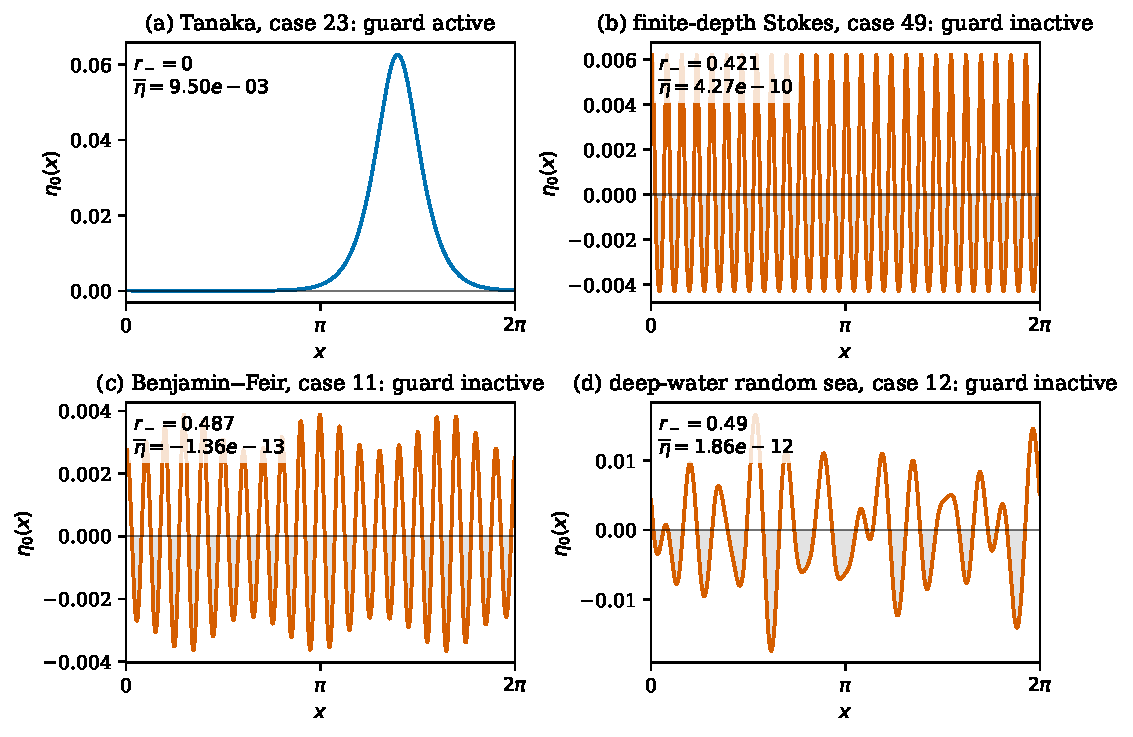
\includegraphics[width=0.96\linewidth]{figures/soliton_selector_examples.pdf}
  \caption{Examples of the initial-condition selector in
  \eqref{eq:soliton-selector}.  Gray shading marks the negative part of each
  surface profile.  The Tanaka profile has negative-energy fraction below
  $10^{-3}$ and positive mean, so the guard is active.  For the three
  non-Tanaka profiles the negative-energy fraction
  exceeds the threshold, so the guard is inactive.  All four cases remain in
  the rollout evaluation.}
  \label{fig:soliton-selector-examples}
\end{figure}

The selector does not estimate oscillation, localization, or family identity.
It tests only the negative-energy fraction and the mean in
\eqref{eq:soliton-selector}; the examples in
\cref{fig:soliton-selector-examples} illustrate the resulting guard state.

For the unnormalized discrete Fourier transform $\widehat\eta_k$, define the
production-band amplitude
\begin{equation}
  A(t)=\frac{1}{N}
  \left(\frac{1}{N}\sum_k
  \mathbf 1_{\{64\leq |k|<128\}}|\widehat\eta_k(t)|^2\right)^{1/2},
  \qquad
  A_{\mathrm{tr}}=\max\!\left(5\times10^{-7},100A(0)\right).
  \label{eq:guard-amplitude}
\end{equation}
The transition is smoothed in logarithmic amplitude,
\begin{equation}
  w(t)=s_0
  \left[1+\exp\!\left(-10\log\frac{A(t)}{A_{\mathrm{tr}}}\right)\right]^{-1}.
  \label{eq:guard-weight}
\end{equation}
We set \(w(t)=0\) when \(A(t)=0\). Thus $w=1/2$ at the threshold, while
$w\approx10^{-10}$ when
$A/A_{\mathrm{tr}}=0.1$. This avoids a discontinuous switch in the numerical
flow.

Once the envelope grows, both canonical variables are multiplied after each
Gauss--Legendre substep by a blended eighth-order Hou--Li-type filter
\cite{hou2007},
\begin{align}
  \sigma_h(k)
  &=\exp\!\left[-0.69
    \left(\frac{|k|}{k_{\mathrm{eff}}(h)}\right)^8\right],
  &k_{\mathrm{eff}}(h)&=\min\!\left(128,\frac{12}{h}\right),
  \label{eq:depth-houli}\\
  \widehat u_k^{\,+}
  &=\left[(1-w)+w\sigma_h(k)\right]\widehat u_k^{\,-},
  &u&\in\{\eta,\xi\}.
  \label{eq:guard-update}
\end{align}
The scale $k_{\mathrm{eff}}h\leq12$ follows the depth scaling of a solitary
wave's horizontal width. It is conservative relative to the truth-spectrum
audit: across the 64 Tanaka reference rollouts, removing content with
$|k|h>8$ changes $\eta$ and $\xi$ by at most
$1.22\times10^{-9}$ and $2.94\times10^{-11}$, respectively, at the 99th
percentile. For the failing depth $h=0.17760$,
$k_{\mathrm{eff}}=67.57$; for the shallow phase-error case,
$12/h>128$, so no additional depth restriction is introduced. The guard is
therefore a conditional spectral viscosity, not a hard global cutoff.

\section{Historical v9 data used for the reported checkpoints}
\label{sec:data}

\subsection{Snapshot construction}

All checkpoint results reported in this manuscript use the historical
\texttt{combined\_dataset\_v9.npz} archive.  The parameterized replacement
dataset discussed below has not yet been used to train a reported model.
Each historical training example is a tuple
\begin{equation}
  (\eta_j,\xi_j,h_j)\longmapsto q_j^\star,
  \label{eq:data-map}
\end{equation}
on the $N=1024$ grid, where $q_j^\star$ is the stored reference target under
that source's generation protocol.  Initial conditions are sampled by wave
family and integrated with the double-precision reference method of
\cref{sec:solver}.  For rollout-derived sources we save multiple trajectory
times, recompute the order-six, pad-eight DNO label in manageable chunks, and
project the label to $|k|\leq128$.  Three static sources (IDs 2--4) instead
store their unfiltered order-six labels.  The mode loss uses only
$1\leq k\leq128$, where the conventions agree; the base loss also supervises
the stored high modes of the static sources.  Fields are stored as 32-bit
arrays, while trajectory generation and label evaluation use float64.

The current v9 dataset contains \num{7633989} snapshots and occupies
approximately \SI{88}{GB}.  Its composition is shown in
\cref{tab:data-composition}.  The families deliberately combine coherent
solutions, spectrally broad random fields, shallow and finite-depth cases, and
nonlinear modulation, broadening the training support beyond solitary-wave
states.

The archive uses fourteen source identifiers to record the generating shard.
In particular, suffixes such as \texttt{g0}, \texttt{g1}, and
\texttt{modal} identify independent generation shards or entry points.  They
do not denote different DNO truncation orders, target definitions, or physical
wave families.  We pool those shards in \cref{tab:data-composition}.

\begin{table}[t]
  \centering
  \caption{Construction-category composition of the historical
  \texttt{combined\_dataset\_v9.npz}, with independent generator shards pooled.}
  \label{tab:data-composition}
  \begin{tabular}{lr@{\qquad}lr}
    \toprule
    Construction category & Snapshots & Construction category & Snapshots\\
    \midrule
    Random sea       & 460,740   & Manufactured harmonic & 500,000\\
    Stokes           & 1,000,000 & Tanaka          & 2,200,000\\
    BF-inspired wavetrain & 2,033,249 & Sparse Fourier packets & 1,440,000\\
    \midrule
    \multicolumn{3}{r}{Total} & 7,633,989\\
    \bottomrule
  \end{tabular}
\end{table}

\subsection{Three roles of the historical construction categories}

The six historical construction categories in \cref{tab:data-composition}
are grouped below according to the states they contribute.  This grouping is
independent of the GPU or generator shard that produced a snapshot.

\paragraph{Coherent traveling and periodic waves (3,200,000 snapshots).}
This group contains both Tanaka and Stokes sources.  Single- and multi-crest
Tanaka conditions are constructed from numerical solitary-wave profiles, with
crest amplitude sampled relative to depth and positions randomized subject to
a minimum separation.  The main shallow set reaches $h=0.01$ and uses an
occupancy-aware upper bound to avoid cutting a broad tail at the periodic
boundary.  The steep addition contributes 200,000 snapshots in
$h\in[0.20,0.35]$ and $a/h\in[0.25,0.45]$.  Deep- and finite-depth Stokes waves
supply periodic states with controlled harmonic content.  Together these
sources resolve coherent nonlinear structure across depth without treating
the deep/finite data partitions as separate physical families.

\paragraph{JCP09-inspired modulated wavetrains (2,033,249 snapshots).}
The historical constructor starts from a fifth-order Stokes carrier and two
sidebands inspired by \cite{xu2009}, but it is not the literal JCP09 initial
condition.  It uses one carrier coefficient for both sidebands, adds empirical
cross terms, and applies the deep-water sideband formula at sampled finite
depths.  Only \(46.7\%\) of the archived parameter draws lie inside the
leading deep-water modulational-instability band.  The three archived shards
are independent samples from this same construction; the suffix
\texttt{modal} does not define a separate family.

\paragraph{Spectral-coverage and perturbation states (2,400,740 snapshots).}
This group combines the manufactured-harmonic, random-sea, and three sparse
Fourier-packet sources.  Manufactured harmonics anchor the small-amplitude
limit, while random seas broaden phase, bandwidth, and local-slope coverage.
The sparse packet sources address the
neighborhood of solitary waves rather than the exact solitary-wave manifold:
they combine one to five Fourier modes while controlling $kh$, $a/h$, and
$ka$.

\subsection{Forward paper-dataset design}

The definitions in this subsection belong to a replacement dataset that has
not yet been used for training.  In particular, they do not describe a
retrospective cleaning of v9 and cannot explain the errors of the checkpoints
reported in this manuscript.  The replacement has four physical families:
fifth-order Stokes states, periodic tangent-Hermite Tanaka profiles, the
equation-(33) sideband construction paired with the project's analytic
fifth-order deep-water carrier, and resolved-band JONSWAP/TMA random seas.
The four physical constructors and their parameter samplers are implemented.
The current family revisions are 2 for Stokes, 3 for Tanaka, and 4 for both
Benjamin--Feir and JONSWAP/TMA.  A revision number is therefore local
to a physical family, rather than a single dataset-wide version number.
Unless an endpoint convention is written explicitly, closed brackets in a
displayed parameter box denote the closure of the continuous support.  The
ordinary floating-point uniform draw uses its lower endpoint and excludes its
upper endpoint.  An endpoint convention written explicitly in an individual
sampling formula---including the half-open phase and center intervals and the
mixed open--closed Benjamin--Feir steepness draw---overrides that default.
These endpoint choices do not change a continuous uniform law, but they are
specified for deterministic regeneration.
For each trajectory family, one common executor runs a
residual-controlled GL2 trajectory with time step \(0.01\), saving a
candidate state every \(0.08\).  JONSWAP/TMA first uses the explicitly
time-dependent adjustment defined below and then starts its autonomous
production trajectory.  A case is retained only when its declared numerical
path returns a complete admissible trajectory on the requested interval.  The
\(0.005\) and \(0.0025\) steps are used only by a separate method-validation
utility; they are not additional production rollouts or retry steps.

Common modules assign a split and parameter category before numerical work and
write one atomic completed-batch artifact containing the family and split, the
ordered parameter-group identifiers, and the accepted row arrays.  A batch slot
with no owned row block denotes a rejected attempt; sampled specifications and
phases, failure reasons, and diagnostic metrics are not persisted.  A resumable
driver continues until the accepted-case quota in every parameter category is
met, replacing a rejected attempt only in its original category.  The fixed
split, family, and attempted-simulation index seed deterministic regeneration.
The training loader uses the preassigned splits and globally shuffles all
accepted training rows.  Unexpected construction or target-evaluation errors
propagate rather than being silently converted into ordinary rejected samples.
The family laws below therefore describe attempted specifications, not the
unconditional law of loader-visible cases.  If \(X\) is a complete attempted
specification in preassigned category \(i\), \(A_f\) is the declared complete
case-acceptance event for family \(f\), and \(w_i\) is the accepted-quota
weight, then the released law is
\begin{equation}
  p_{\mathrm{release}}(i,x)
  =w_i\,p_{\mathrm{proposal}}(x\mid i,A_f=1).
  \label{eq:paper-accepted-law}
\end{equation}
For Stokes, \(A_f\) comprises declared static support, a finite state, positive
water column, and a finite target.  For Tanaka, it comprises declared
construction support followed by complete autonomous-trajectory acceptance;
for Benjamin--Feir, initial-state validity followed by complete autonomous-
trajectory acceptance.  For JONSWAP/TMA, it comprises initial construction and
graph validity followed by nonlinear adjustment and complete autonomous-
trajectory acceptance.  Thus the quotas preserve the declared category
marginals, not the unconditioned proposal law within a category.  This is a
statement about how the release is constructed; it does not by itself assert a
measured within-category shift for every family.  No retrospective parameter
cutoff is applied.  The loader-facing manifest and row map record the selected
shards, split totals, and case-to-row ownership; they do not persist numerical-
configuration or source hashes.  The release described here selects Stokes
revision 2, Tanaka revision 3, Benjamin--Feir revision 4, and JONSWAP/TMA
revision 4.

An earlier generator-revision-1 complete transaction smoke test used a reduced
wiring contract:
64 spatial grid points, Craig--Sulem order zero, padding factor one, largest
delivered wavenumber 16, and the former paired \(0.04/0.02\) validation path.
One Tanaka case, one Benjamin--Feir case, and one random-sea case were each
accepted to a quota of one case; each committed three rows, and all nine rows
were finite when read by the training loader.  This reduced calculation tests
the transaction and loader, not the current family-revision executors, the
paper target, the long-horizon numerical contract, or a population acceptance
rate.  The current numerical paths have focused software-test coverage.
A former revision-2 104-category trajectory pilot predates the Tanaka
revision-3 support and numerical contract and remains historical software-path
evidence.  The present family specifications contain 108 categories: four
Stokes, eleven Tanaka, 66 Benjamin--Feir, and 27 JONSWAP/TMA.  The exact
revision-3 Tanaka pilot passed all eleven Tanaka categories.  The revision-4
Benjamin--Feir exact-source gate passed all 66 categories, and its production
splits are complete at 16384 training cases and 1024 cases in each of
validation and test.  The revision-4 JONSWAP/TMA source was tested more
broadly: a predeclared gate retained 540 trajectories, 20 in each of its 27
categories, from 548 attempts.  Its observed rejection rate was therefore
\(8/548=1.46\%\), below the predeclared two-percent bound.  This was the
completed constructor-adoption criterion, not a bulk release threshold.  The
subsequent revision-4 bulk release is complete: it retained \num{18432} cases
from \num{18726} attempts, recorded \num{294} zero-row rejections, and stored
\num{294912} rows.

The revision-2 Stokes splits are complete at the same accepted-case counts as
Benjamin--Feir.  A historical Tanaka run produced 2048 training, 1024
validation, and 1024 test cases, but those trajectories are excluded from the
paper dataset.  The old solitary-wave solve could not realize crest amplitudes
below \(9.9478\times10^{-4}\); 64 of the 4096 historical cases contain one
requested component below this floor.  The smallest requested component was
inflated by a factor \(41.27\) after periodic construction and projection.
The corrected solve uses \(q_c^{\max}=1-10^{-12}\), 48 bisections, and checks
that every realized crest height matches its request.  The corrected
revision-3 release is a fresh deterministic population with 16384
training cases and 1024 cases in each of validation and test.  It does not
reuse the historical random specifications, and no old and corrected Tanaka
rows are mixed.  All \num{18432} corrected attempts were accepted and stored
\num{3686400} rows.

\paragraph{One frozen learning target.}
Let the spatial period be $L=2\pi$, let $N=1024$, and let
$\Delta x=L/N$ and $x_\ell=\ell\Delta x$, $\ell=0,\ldots,N-1$, be the grid
spacing and nodes.  For a periodic grid function $u$, let $P_K u$ retain its
Fourier modes with $|k|\leq K$, where $K=128$, and let $P_K^\circ u$ also set
the zero Fourier mode to zero.  We
write $\G_M^{N,p}(\eta;h)\xi$ for the order-$M$ Craig--Sulem approximation on
$N$ points with product-padding factor $p$, surface elevation $\eta$, surface
potential $\xi$, and depth $h>0$.  The target is fixed to
\begin{equation}
  q_{\mathrm{ref}}(\eta,\xi;h)
  =
  P_K^\circ\!\left[
    \G_{6}^{1024,8}(P_K\eta;h)(P_K\xi)
  \right].
  \label{eq:forward-dataset-target}
\end{equation}
Thus both inputs are restricted before evaluation, and the output is
restricted and made mean zero afterward.  The target is evaluated in float64;
the three fields $\eta$, $\xi$, and $q_{\mathrm{ref}}$ are stored in float32,
while depth and retained time are stored in float64.  The sampled parameters
from which a row was constructed are not stored.
Thus the mean-zero statement is exact for the float64 target and is preserved
in the stored array only to float32 rounding error.
Static Stokes states use exactly \cref{eq:forward-dataset-target}, rather than
the unfiltered labels in some historical v9 sources.  The paper generator fixes
$L,N,K,M,p$ and the evaluation precision in its numerical settings; the completed
batches do not record target-configuration or source hashes.
The three trajectory families have internal evolution contracts specified
below, but all deliver the same target in
\cref{eq:forward-dataset-target}.

JONSWAP/TMA is evolved on a larger grid than the stored target.  To specify
the transfer without an FFT-normalization ambiguity, for a field sampled on
\(N'\) points define
\begin{equation}
  \widehat f_k^{(N')}
  =\frac1{N'}\sum_{j=0}^{N'-1}
    f\!\left(\frac{2\pi j}{N'}\right)e^{-2\pi i jk/N'}.
  \label{eq:paper-normalized-fourier-coefficient}
\end{equation}
At each retained JONSWAP/TMA time, the coefficients of \(\eta\) and \(\xi\)
with \(|k|\le128\) are copied from the 2048-point internal grid and
reconstructed on the 1024-point grid.  Equation
\eqref{eq:forward-dataset-target} is then evaluated from those reconstructed
fields.  The internal value of \(G(\eta;h)\xi\) is never transferred between
grids; recomputing it is necessary because the stored label is the declared
1024-point order-six operator, not the order-four operator used for evolution.

\paragraph{Static fifth-order Stokes states.}
Let $n\geq1$ be an integer carrier mode, $k=2\pi n/L$ its wavenumber,
$a>0$ the amplitude parameter in Fenton's fifth-order expansion
\cite{fenton1985}, $h>0$ the depth, and
$\phi\in[0,2\pi)$ a spatial phase.  The finite- and deep-water coefficient
tables are two parameter branches of the same fifth-order family.  In either
branch the constructor evaluates the state directly at
\begin{equation}
  \theta=kx+\phi,
  \qquad \phi\sim\operatorname{Unif}[0,2\pi).
  \label{eq:paper-stokes-phase}
\end{equation}
No sampled time is used as a substitute for $\phi$: changing $a$ changes the
nonlinear temporal frequency, whereas \cref{eq:paper-stokes-phase} preserves
the requested spatial translation.  The spatial mean of $\xi$ is removed to
fix the irrelevant constant-potential gauge.

The common amplitude interval is
\begin{equation}
  0.000766\leq a\leq0.011494.
  \label{eq:paper-stokes-amplitude}
\end{equation}
In the finite-depth branch,
\begin{equation}
  n\in\{14,\ldots,26\},\qquad
  0.02\leq h\leq1.5,\qquad
  0.5\leq kh\leq5,
  \label{eq:paper-stokes-finite-support}
\end{equation}
whereas the deep-water branch uses
\begin{equation}
  n\in\{1,\ldots,20\},\qquad
  4\leq h\leq50,\qquad
  kh\geq5.
  \label{eq:paper-stokes-deep-support}
\end{equation}
The steepness $ka$ is assigned to one of the two categories
\begin{equation}
  0.005\leq ka<0.03,
  \qquad
  0.03\leq ka\leq0.15.
  \label{eq:paper-stokes-cells}
\end{equation}
The finite/deep branches crossed with these two intervals form four parameter
categories.  Within an assigned category, the sampler first enumerates the carrier
modes for which the branch, depth, amplitude, and steepness intervals have
nonempty intersection, and chooses one of those modes uniformly.  It then
draws \(h\) log-uniformly on the mode-conditioned depth interval, draws
\(\phi\) uniformly on \([0,2\pi)\), and draws \(a\) uniformly from the
intersection of \cref{eq:paper-stokes-amplitude} with the assigned steepness
interval.

The finite-depth branch has an additional support condition.  Write its
elevation as
\begin{equation}
  \eta_5(\theta)=\sum_{m=1}^{5}E_m\cos(m\theta),
  \label{eq:paper-stokes-harmonics}
\end{equation}
where $E_m$ is the coefficient of the $m$th harmonic.  Let
$H=\max_\theta\eta_5(\theta)-\min_\theta\eta_5(\theta)$ be the exact
crest-to-trough height, and let $H_{4096}$ be the corresponding maximum minus
minimum over 4096 equally spaced values of $\theta$.  Define
\begin{equation}
  H_+
  =
  H_{4096}
  +\frac{1}{4}\left(\frac{2\pi}{4096}\right)^2
    \sum_{m=1}^{5}m^2|E_m|,
  \qquad
  \mathrm{Ur}_+
  =
  \frac{H_+\lambda^2}{h^3},
  \qquad
  \lambda=\frac{2\pi}{k}.
  \label{eq:paper-stokes-ursell}
\end{equation}
Since $|\eta_5''|\leq\sum_{m=1}^5m^2|E_m|$, Taylor's theorem at the true
maximum and minimum gives $H\leq H_+$.  The finite-depth sampler therefore
requires the conservative condition $\mathrm{Ur}_+\leq26$.  This is a
restriction on the parameter support of the fifth-order family, not a filter
trained on integration failures.  Fenton identifies the corresponding
shallow-water expansion parameter for fifth-order Stokes theory
\cite{fenton1985}, and Zhao, Wang, and Liu use $\mathrm{Ur}=26$ to separate
the fifth-order Stokes and shallower cnoidal regimes \cite{zhao2024}.
The coefficient implementation follows the fifth-order formula checked
against Zhao and Liu \cite{zhao2022}.  The deep-water branch instead requires
$kh\geq5$.

\paragraph{Seeded sampling.}
Let $s$ be the root seed fixed by the data split, let $f$ identify the physical
family, and let $i$ be the attempted-simulation index.  A simulation uses NumPy
PCG64 initialized from $(s,f,i)$.  The four
categories are the finite/deep branches crossed with the two intervals in
\cref{eq:paper-stokes-cells}.  Requested accepted-case counts are divided
among these categories by quotient and remainder before any state is constructed.
This is a seeded stratified pseudorandom construction, not a low-discrepancy
sequence.  A successful proposal holds its realized mode, amplitude, depth,
phase, branch, and category only long enough to construct its rows; these
values can instead be regenerated from the split, family, and attempt seed.

If a finite-depth amplitude draw violates
$\mathrm{Ur}_+\leq26$, only the amplitude is redrawn, uniformly from the same
category intersection.  Its mode, depth, phase, and category remain fixed.  The case
may make at most 1000 additional amplitude draws.  Intermediate rejected
amplitudes and their values of $\mathrm{Ur}_+$ are not persisted.  If the
redraw allowance is exhausted, the sampler returns no state and the batch slot
owns no rows; generation then fills the remaining
accepted-case quota from a later attempt in the same category.

\paragraph{Static archive and replay checks.}
These checks concern only the implemented Stokes component of the replacement
dataset.  A 16-case finite-depth archive contained eight cases from each category
in \cref{eq:paper-stokes-cells}, required three same-category redraws, and had
$\max\mathrm{Ur}_+=18.0578589$.  A separate 16-case deep archive was finite
and had $\min kh=10.0678$.  Its category counts were nine and seven because some
carrier modes admitted only one steepness category; the subset admitting both remained
balanced to within one.  Re-evaluating
\cref{eq:forward-dataset-target} from the stored float64 parameters and then
converting the fields to float32 reproduced both archives bit for bit.  A
synthetic interruption after two batches likewise resumed to the same 30
ordered archive entries, byte for byte, as an uninterrupted 32-case run.  In
a 20,000-case finite-depth sampling stress with root seed 20260725 and stream
zero, the two category counts were 10,000 and 10,000, the largest accepted value
was $\mathrm{Ur}_+=25.9724665$, the largest redraw count was 56, and no case
exhausted the cap.  A separate forced-exhaustion quota test committed the
attempt as a zero-row out-of-support rejection and scheduled a
replacement in the same category.

The common static transaction was also exercised at the exact target
resolution $(N,M,p,K)=(1024,6,8,128)$ in float64.  One validation attempt was
assigned to each finite/deep and low/moderate category, and its complete
specification was written before construction.  All four attempts had finite
input and target fields, positive water column, no support violation, and no
failed required quality check.  The transaction therefore committed one
$t=0$ row per case and constructed the split-aware dataset view.  This
accepted-quota calculation accepted all four attempts and checks the exact
implementation path; it does not estimate a population acceptance
probability.

\paragraph{Periodic tangent-Hermite Tanaka states.}
Let $\alpha=a/h>0$ be the ratio of crest amplitude $a$ to depth $h$.
Following Tanaka's solitary-wave formulation \cite{tanaka1986}, a unit-depth
solve at amplitude ratio $\alpha$ returns a dimensionless surface profile
$\bar\eta_\alpha(X)$, a tabulated surface angle $\theta_\alpha(X)$, and a
Froude number $F_\alpha$.  Xu and Guyenne also use a solitary wave computed
by Tanaka's method \cite{xu2009}.  The tangent-Hermite interpolation,
periodization, multi-crest superposition, and parameter sampling below are
choices of the present dataset; they are not parts of either cited
solitary-wave construction.  Here $X$ is the dimensionless horizontal
coordinate, and
\begin{equation}
  \frac{\dd\bar\eta_\alpha}{\dd X}(X)
  =\tan\theta_\alpha(X).
  \label{eq:paper-tanaka-slope}
\end{equation}
Before interpolation, the constructor verifies that both endpoint elevations
and the endpoint and crest tangents differ from zero by at most $10^{-12}$,
then sets those quantities exactly to zero.  The corrected tabulated profile
is extended by zero outside its finite tabulation interval.  Between adjacent
tabulation points, the constructor uses the unique cubic polynomial matching
both endpoint values of $\bar\eta_\alpha$ and both endpoint values of
$\tan\theta_\alpha$.  Thus ``tangent-Hermite'' specifies the interpolation,
not an additional wave model.  The physical derivative is correctly scaled
because
\begin{equation}
  \partial_x\!\left[
    h\bar\eta_\alpha\!\left(\frac{x-x_0+rL}{h}\right)
  \right]
  =
  \frac{\dd\bar\eta_\alpha}{\dd X}
  \!\left(\frac{x-x_0+rL}{h}\right).
  \label{eq:paper-tanaka-scaled-slope}
\end{equation}

For a crest centered at $x_0\in[0,L)$, define the periodic elevation
\begin{equation}
  \eta_{\alpha,h,x_0}(x)
  =
  h\sum_{r\in\mathbb Z}
  \bar\eta_\alpha\!\left(\frac{x-x_0+rL}{h}\right).
  \label{eq:paper-tanaka-periodization}
\end{equation}
Only finitely many terms in \cref{eq:paper-tanaka-periodization} are nonzero
at a given $x$, because the extended profile has finite support.  The
implementation sums every periodic image whose support intersects $[0,L)$;
it does not retain only the nearest three images.  The sum is evaluated on an
$8N$-point grid and Fourier-restricted to the $N$-point grid.

Let $g>0$ be gravitational acceleration, let
$c_\alpha=F_\alpha\sqrt{gh}$ be the unsigned wave speed, and let
$s\in\{-1,1\}$ denote the direction of travel.  Write
$\eta_x=\partial_x\eta_{\alpha,h,x_0}$.  The traveling-wave relation first
defines
\begin{equation}
  r_{\alpha,h,x_0,s}(x)
  =
  s\left[
    c_\alpha-
    \sqrt{(1+\eta_x(x)^2)
      (c_\alpha^2-2g\eta_{\alpha,h,x_0}(x))}
  \right].
  \label{eq:paper-tanaka-potential-derivative}
\end{equation}
Define the expression under the square root by
\begin{equation}
  \mathcal R_{\alpha,h,x_0}(x)
  =
  (1+\eta_x(x)^2)
  (c_\alpha^2-2g\eta_{\alpha,h,x_0}(x)).
  \label{eq:paper-tanaka-radicand}
\end{equation}
The constructor requires the nodewise condition
$\min_\ell\mathcal R_{\alpha,h,x_0}(x_\ell)\geq0$ and treats an attempted component
that violates this condition as inadmissible; it does not replace a negative
value by zero.  For the fixed upper-steepness, seam-centered test case, the
initial value is
$\min_\ell\mathcal R_{\alpha,h,x_0}(x_\ell)/c_\alpha^2=0.372151$.  Hence the clipping
in the old writer did not change that particular initial condition.  This
single positive margin does not establish the condition for the full
population.

Let $\widehat r_n$ be the Fourier coefficient of
$r_{\alpha,h,x_0,s}$ at wavenumber $k_n=2\pi n/L$.  The periodic,
zero-mean surface potential is defined by
\begin{equation}
  \widehat\xi_n
  =
  \begin{cases}
    \widehat r_n/(ik_n),&n\ne0,\\
    0,&n=0.
  \end{cases}
  \label{eq:paper-tanaka-potential}
\end{equation}
Consequently $\partial_x\xi=r_{\alpha,h,x_0,s}-\widehat r_0$; subtracting
the constant $\widehat r_0$ is necessary for a periodic antiderivative.

A case with $m\geq1$ crests has parameters
$(h,m,\alpha_j,x_j,s_j)_{j=1}^m$ and initial state
\begin{equation}
  (\eta_0,\xi_0)
  =
  P_K\sum_{j=1}^{m}
  \left(
    \eta_{\alpha_j,h,x_j},
    \xi_{\alpha_j,h,x_j,s_j}
  \right).
  \label{eq:paper-tanaka-state}
\end{equation}
For $m>1$, \cref{eq:paper-tanaka-state} is a superposition of separately
constructed solitary-wave profiles, not an exact steady multi-solitary-wave
solution.
The sharp $P_K=P_{128}$ map in \cref{eq:paper-tanaka-state} is applied once
before time integration.  Revision 3 then embeds this state in the larger
$|k|\leq256$ evolution space by setting modes $129\leq|k|\leq256$ initially
to zero.  Nonlinear evolution may populate those workspace modes, but the
initial-value problem is exactly the sharp-$P_{128}$ problem used in the
resolution calculation below.
For two centers $x_i,x_j\in[0,L)$, define their periodic distance by
\begin{equation}
  d_L(x_i,x_j)
  =
  \min_{r\in\mathbb Z}|x_i-x_j+rL|.
  \label{eq:paper-periodic-distance}
\end{equation}
The centers must satisfy $d_L(x_i,x_j)\geq3h$ whenever $i\ne j$.

The amplitudes are sampled before the depth.  In a main group, define the
total dimensionless amplitude
$\alpha_\Sigma=\sum_{j=1}^m\alpha_j$ and draw
$\alpha_\Sigma\sim\operatorname{Unif}[0.10,0.35]$.  Draw nonnegative weights
$(\lambda_1,\ldots,\lambda_m)$ uniformly on the simplex
$\sum_j\lambda_j=1$, equivalently from
$\operatorname{Dirichlet}(1,\ldots,1)$, and set
$\alpha_j=\alpha_\Sigma\lambda_j$.  For $m=1$, this means
$\lambda_1=1$.  In a steep group, draw the single amplitude ratio
$\alpha_1\sim\operatorname{Unif}[0.25,0.45]$.  In both groups, define
\begin{equation}
  \alpha_{\max}=\max_{1\leq j\leq m}\alpha_j.
  \label{eq:paper-tanaka-maximum-amplitude}
\end{equation}

The depth interval is then restricted before a profile is constructed.  The
small-amplitude KdV profile has the form
\begin{equation}
  \frac{\eta(x)}{h}
  \approx
  \alpha_{\max}\operatorname{sech}^2\!\bigl(\kappa(x-x_0)\bigr),
  \qquad
  \kappa=\frac{\sqrt{3\alpha_{\max}}}{2h},
  \label{eq:paper-tanaka-kdv-width}
\end{equation}
where $\operatorname{sech}z=1/\cosh z$ and $\kappa$ is an inverse length.
We use $\kappa$ only as a small-amplitude KdV inverse-width proxy for the
narrowest component.  It is not the exact width of a Tanaka profile.  With
the delivered cutoff $K=128$, define the number of delivered wavenumbers per
proxy inverse width by
\begin{equation}
  R=\frac{128}{\kappa}
   =\frac{256h}{\sqrt{3\alpha_{\max}}}.
  \label{eq:paper-tanaka-resolution-ratio}
\end{equation}
Tanaka revision 3 requires $R\geq10$.  This threshold is a numerical design
choice established by the resolution tests below; it is not a condition
stated in \cite{tanaka1986} or \cite{xu2009}.

The proxy first arose from a retrospective resolution audit, rather than from
a fitted rejection statistic.  We reconstructed 256 tangent-Hermite proposals
before their sharp $P_{128}$ projection.  All eleven cases that exceeded the
historical $K_{\mathrm{evol}}=224$ Hamiltonian-drift diagnostic had $R<8$.
The 210 cases with $R\geq8$ contained none of those diagnostic failures, and
their largest raw-to-$P_{128}$ relative root-mean-square errors were
$6.80\times10^{-5}$ for $\eta$ and $4.47\times10^{-6}$ for $\xi$.  By
comparison, the unrelated fixed restriction $h\geq0.025$ admitted a larger
maximum $\eta$ projection error, $4.33\times10^{-4}$.  These observations
identify under-resolved input width as the mechanism; the full-horizon panel
below, not the historical Hamiltonian threshold, determines the revision-3
support.

For a base lower depth $b>0$, define
\begin{equation}
  h_-(\alpha;b)
  =\max\!\left\{b,\frac{10\sqrt{3\alpha}}{256}\right\}.
  \label{eq:paper-tanaka-depth-lower-bound}
\end{equation}
After the amplitudes have been drawn, sample $U_h\sim\operatorname{Unif}[0,1]$
and set
\begin{equation}
  h=h_-^{\,1-U_h}h_+^{\,U_h},
  \label{eq:paper-tanaka-geometric-depth}
\end{equation}
where $h_-=h_-(\alpha_{\max};0.01)$ and $h_+=0.30$ in a main group, while
$h_-=h_-(\alpha_1;0.20)$ and $h_+=0.35$ in a steep group.  Thus $h$ is
log-uniform on the conditional interval $[h_-,h_+]$.  The resolution term in
\cref{eq:paper-tanaka-depth-lower-bound} is at most $0.0454$ on the steep
amplitude interval, so the steep lower bound remains $0.20$ and the
resolution restriction is inactive there.  The resulting supports are
therefore
\begin{align}
  &m\in\{1,2,3\},\quad
    \alpha_\Sigma\in[0.10,0.35],\quad
    h\in[h_-(\alpha_{\max};0.01),0.30]
    &&\text{(main)},
  \label{eq:paper-tanaka-main-support}\\
  &m=1,\quad
    \alpha_1\in[0.25,0.45],\quad
    h\in[0.20,0.35]
    &&\text{(steep)}.
  \label{eq:paper-tanaka-steep-support}
\end{align}
Equal increments of $U_h$ give equal multiplicative changes of depth.  This is
a coverage rule for the numerical experiment, not a probability model for
physical water depths.  In a deterministic million-draw audit for each
$m=1,2,3$, the $R\geq10$ condition removed $28.55\%$ of the former
independent-depth law after weighting the nine main categories by their
$2:3:4$ category counts.  The median depths for $m=1,2,3$ were respectively
$0.0973$, $0.0902$, and $0.0857$, and their 95th percentiles were $0.2680$,
$0.2659$, and $0.2647$.

For each case let
\begin{equation}
  q=\#\{j:s_j=+1\}
  \label{eq:paper-tanaka-right-count}
\end{equation}
be the number of right-moving crests.  The three choices of $m$ in
\cref{eq:paper-tanaka-main-support}, crossed with
$q=0,\ldots,m$, give nine parameter categories.  The steep support in
\cref{eq:paper-tanaka-steep-support}, crossed with $q=0,1$, gives two more.
Thus the Tanaka family has eleven parameter categories.

The requested Tanaka accepted-case count is divided equally across these
eleven categories, up to the unavoidable difference of one case when the
total is not divisible by eleven.  Conditional on $q$, the sampler chooses
uniformly which $q$ of the $m$ exchangeable crest labels have sign $+1$; all
remaining signs are $-1$.  Hence left and right directions remain balanced
marginally in the ideal equal-category population, while the direction
compositions $q=0,\ldots,m$ receive equal coverage instead of their former
binomial frequencies under independent fair signs.  For a finite quota, the
quotient--remainder assignment changes category counts by at most one and may
therefore introduce a one-case direction imbalance.  In particular, the
fixed category order gives a quota of 1024 one extra left-moving one-crest
case.  This law also gives more aggregate Tanaka weight to
$m=2$ and $m=3$, because they have three and four distinct direction
compositions, respectively.  The corrected full-size Tanaka production is
complete.  Its historical 4096-case predecessor and its eleven-case
revision-3 pilot are excluded from the replacement-dataset view.

Tanaka revision 3 retains the eleven direction-aware categories introduced in
revision 2, but changes the amplitude--depth draw order, the admissible depth
support, and the internal numerical contract.  Earlier Tanaka revision-1 and
revision-2 smokes, dry runs, and pilot artifacts remain historical
constructor or transaction evidence; they cannot be resumed into a
revision-3 run.  Benjamin--Feir and JONSWAP/TMA use revision 4; static Stokes
remains at revision 2.

To sample centers without a translation bias, let
$(w_1,\ldots,w_m)$ have the same uniform-simplex law and set the cyclic gaps
to
\begin{equation}
  g_j=3h+(L-3mh)w_j,\qquad j=1,\ldots,m.
  \label{eq:paper-tanaka-gap-law}
\end{equation}
A uniform global rotation places the resulting point set on the periodic
domain.  Directions are then assigned according to the category as described
above.  In a steep group, the center uses this same uniform rotation and the
direction is fixed by $q\in\{0,1\}$.  The separation is always feasible on
the declared support because $3mh\leq2.7<2\pi=L$.  Thus separation and
translation symmetry are enforced before integration.

The population sampler and ordered batch adapter are implemented.  The
sampled parameters are held only during construction and can be regenerated
from the split, family, and attempt seed.  The potential routine
transfers the computed radicand to the host once before taking the square root
and introduces no clipping tolerance.  An everywhere-finite, positive-speed
component with a negative radicand is a declared support rejection: it
contributes no rows and is replaced in the same category.  A nonfinite radicand,
a nonpositive or nonfinite computed speed, or an unexpected exception remains
an implementation error and stops the run.
In the historical reduced paired calculation described above, the Tanaka
attempt was accepted, committed three finite rows, and was finite when read by
the training loader.  This is transaction evidence at the reduced contract,
not evidence about the current Tanaka trajectory executor or the Tanaka
population.

Tanaka revision 3 evolves an internal band
$|k|\leq K_{\mathrm{evol}}$ with $K_{\mathrm{evol}}=256$.  Let
$\widehat\eta_{0,k}$ and $\widehat\xi_{0,k}$ be the Fourier coefficients of
the sharp-$P_{128}$ state in \cref{eq:paper-tanaka-state}.  The internal state
is initialized by the zero-filled lift
\begin{equation}
  \bigl(\widehat\eta_k(0),\widehat\xi_k(0)\bigr)
  =
  \begin{cases}
    \bigl(\widehat\eta_{0,k},\widehat\xi_{0,k}\bigr),&|k|\leq128,\\
    (0,0),&128<|k|\leq256.
  \end{cases}
  \label{eq:paper-tanaka-zero-filled-lift}
\end{equation}
Thus no discarded raw-profile mode is supplied to the wider evolution at
$t=0$; modes above 128 can arise only from the subsequent dynamics.  The
$K_{\mathrm{evol}}=224$ comparison arm uses the same construction with upper
limit 224.  After every completed GL2 step, the Fourier coefficients
$\widehat\eta_k$ and $\widehat\xi_k$ are multiplied by
\begin{equation}
  \sigma_k
  =\exp\!\left[-36\left(\frac{|k|}{256}\right)^{36}\right].
  \label{eq:paper-tanaka-hou-li-filter}
\end{equation}
This is the power-36 Hou--Li filter \cite{hou2007} used on both canonical
variables, with the parameters of \cite[Eq.~(29)]{xu2009}.  The
$K_{\mathrm{evol}}=224$ comparison arm replaces 256 in
\cref{eq:paper-tanaka-hou-li-filter} by 224.  At each saved time, the delivered
state is
$(P_{128}\eta,P_{128}\xi)$ and the delivered label is
$q_{\mathrm{ref}}$ from \cref{eq:forward-dataset-target}.  Modes
$129\leq|k|\leq256$ therefore stabilize the internal evolution but are not
stored as inputs or labels for learning.
This sharp \(P_{128}\) initial projection, zero-filled lift to
\(K_{\mathrm{evol}}=256\), post-step Hou--Li multiplier, and final
\(P_{128}\) delivery is the exact revision-3 contract used by the pilot.  The
excluded historical July training shards used the same numerical contract but
are not part of the fresh paper dataset.

The resolution choice was tested on nine one-crest cases.  Their amplitude
ratios were $\alpha\in\{0.225,0.30,0.35\}$, and their resolution ratios were
$R\in\{6,8,10\}$.  Each case was evolved from the same bit-identical
$P_{128}$ initial state with
$K_{\mathrm{evol}}=224$ and 256 through $T=200$.  Define the dimensionless
delivered fields
\begin{equation}
  \widetilde\eta_J(t)=\frac{P_{128}\eta_J(t)}{h},\qquad
  \widetilde\xi_J(t)=\frac{P_{128}\xi_J(t)}{h\sqrt{gh}},\qquad
  \widetilde q_J(t)
  =\frac{q_{\mathrm{ref}}(\eta_J(t),\xi_J(t);h)}{\sqrt{gh}},
  \label{eq:paper-tanaka-dimensionless-comparison-fields}
\end{equation}
where $J\in\{224,256\}$ is the internal cutoff and
$(\eta_J,\xi_J)$ is that arm's internal state.  For
$u\in\{\widetilde\eta,\widetilde\xi,\widetilde q\}$, define the reported
cross-resolution error by
\begin{equation}
  \epsilon_u
  =\max_t
  \frac{\lVert u_{224}(t)-u_{256}(t)\rVert_{2,N}}
       {\max_s\lVert u_{256}(s)\rVert_{2,N}+10^{-12}},
  \qquad
  \lVert v\rVert_{2,N}^2
  =\frac{1}{N}\sum_{\ell=0}^{N-1}|v(x_\ell)|^2.
  \label{eq:paper-tanaka-cross-resolution-error}
\end{equation}
The three fields are nondimensionalized before the additive $10^{-12}$ floor
is applied.  Write $\epsilon_\eta$, $\epsilon_\xi$, and $\epsilon_q$ for
\cref{eq:paper-tanaka-cross-resolution-error} evaluated with
$u=\widetilde\eta$, $\widetilde\xi$, and $\widetilde q$, respectively.  The
audit also checked the analogous full-history RMS error.  To measure whether
hidden state modes alter the delivered operator, define
\begin{equation}
  d_J(t)
  =P_{128}^\circ\!\left[
    \G_6^{1024,8}(\eta_J(t);h)\xi_J(t)
  \right]
  -q_{\mathrm{ref}}(\eta_J(t),\xi_J(t);h),
  \label{eq:paper-tanaka-hidden-band-defect}
\end{equation}
where $(\eta_J,\xi_J)$ is the internal state of arm $J$.  Its reported closure
error is
\begin{equation}
  C_J
  =\max_t
  \frac{\lVert d_J(t)\rVert_{2,N}}
       {\max_s\lVert q_{\mathrm{ref}}(\eta_J(s),\xi_J(s);h)\rVert_{2,N}
        +10^{-12}}.
  \label{eq:paper-tanaka-hidden-band-closure}
\end{equation}

All three $R=6$ controls failed the predeclared $10^{-3}$ comparison; their
worst operator error was $\epsilon_q=9.36\times10^{-3}$ and
their worst closure error was $2.91\times10^{-3}$.  All three $R=8$ cases
passed, but their worst errors were
$(\epsilon_\eta,\epsilon_\xi,\epsilon_q)
=(1.87\times10^{-4},1.29\times10^{-5},7.34\times10^{-4})$ and
$\max_J C_J=6.31\times10^{-4}$.  At $R=10$, these values fell to
$(2.94\times10^{-5},1.62\times10^{-6},1.35\times10^{-4})$ and
$1.40\times10^{-4}$.  Each arm completed all 20,000 GL2 time steps, and both
coupled implicit stage equations converged at every step.  The largest
delivered-$P_{128}$ Hamiltonian drift among the $R=10$
arms was $2.99\times10^{-8}$; this value is reported only as a numerical
diagnostic and is not a production acceptance condition.  We therefore use
the round margin $R\geq10$ and the exact two-times internal band
$K_{\mathrm{evol}}=256$ in Tanaka revision 3.

\paragraph{Equation-(33) Benjamin--Feir states.}
This family is restricted to deep water.  Let $n_c\in\mathbb N$ be the
carrier-mode index, let $\Delta n\in\mathbb N$ be the symmetric sideband
offset with $\Delta n<n_c$, let $\varepsilon_c>0$ be the steepness of the
first elevation harmonic, let $\rho>0$ be the sideband-to-carrier amplitude
ratio, and let $x_0\in[0,L)$ be a global spatial translation.  Thus
$\varepsilon_c$ is not defined from half the crest-to-trough wave height.
Define
\begin{equation}
  k_c=\frac{2\pi n_c}{L},\qquad
  k_-=\frac{2\pi(n_c-\Delta n)}{L},\qquad
  k_+=\frac{2\pi(n_c+\Delta n)}{L},\qquad
  a=\frac{\varepsilon_c}{k_c}.
  \label{eq:paper-bf-wavenumbers}
\end{equation}
The sideband ansatz follows equation~(33) of Xu and Guyenne, who in turn
follow Dommermuth and Yue \cite{dommermuth1987,xu2009}.  Their published test
uses, in the present notation,
\begin{equation}
  (n_c,\Delta n,\varepsilon_c,\rho,\theta)
  =
  (9,2,0.13,0.10,-\pi/4),
  \qquad L=2\pi,\qquad g=1.
  \label{eq:paper-bf-published-tuple}
\end{equation}
It also uses a numerically computed exact steady Stokes carrier.  The
construction below is our randomized generalization over 66 integer
mode-pair categories, not a reproduction of that single parameter tuple.

Let $y=x-x_0$, and let $(\eta_c(y),\xi_c(y))$ denote the project's analytic
fifth-order deep-water Stokes formula, with carrier phase zero in this
translated coordinate and first elevation harmonic of amplitude $a$.  This
analytic fifth-order carrier is an approximation to the published exact
steady carrier; it is not the Xu--Guyenne carrier itself.  Both sidebands use
the fixed relative phase $\theta=-\pi/4$ from the cited calculation.

With $\eta_0$ evaluated before $\xi_0$, the implemented sideband construction
is
\begin{align}
  \eta_0(x)
  &=
  \eta_c(y)+\rho a\left[
    \cos(k_-y+\theta)+\cos(k_+y+\theta)
  \right],
  \notag\\
  \xi_0(x)
  &=
  \xi_c(y)+\rho a\left[
    \sqrt{\frac{g}{k_-}}\,e^{k_-\eta_0(x)}\sin(k_-y+\theta)
    +
    \sqrt{\frac{g}{k_+}}\,e^{k_+\eta_0(x)}\sin(k_+y+\theta)
  \right].
  \label{eq:paper-bf-state}
\end{align}
The spatial mean of $\xi_0$ is removed after
\cref{eq:paper-bf-state}.  Both sidebands use the same $\rho$ and $\theta$;
there are no empirical cross terms.  Translating the complete state changes
neither the relative phases nor the resonant quartet phase, which remains
$\theta+\theta-2(0)=-\pi/2$.  The numerical depth is
$h=5L/(2\pi)$, so the first nonzero wavenumber $k_1=2\pi/L$ satisfies
$k_1h=5$.

For a proposed pair, define the normalized sideband location and a
focused-envelope steepness proxy by
\begin{equation}
  \beta
  =\frac{\Delta n/n_c}{2\sqrt{2}\,\varepsilon_c},
  \qquad
  \varepsilon_f
  =\varepsilon_c\left(1+2\sqrt{1-\beta^2}\right).
  \label{eq:paper-bf-band}
\end{equation}
Benjamin and Feir give the historical deep-water instability
condition~\cite{benjaminfeir1967}.  In the present normalization,
equation~(4.6) of Andrade and Stuhlmeier gives $0<\beta<1$, while their
equations~(5.7)--(5.11) give the Akhmediev-breather correspondence and the
peak-envelope amplification factor
$1+2\sqrt{1-\beta^2}$~\cite{andrade2023}.  We use that factor only to define
the scalar population-screening proxy above.  Yang and Liu use
$\varepsilon_c=0.10$, five-percent sidebands, and the maximum-growth
frequency coordinate $\Delta\omega/(\omega_c\varepsilon_c)=1$
\cite[Sec.~4.3.1]{yangliu2024}.  Under the leading deep-water narrowband
relation $\Delta k/k_c\simeq2\Delta\omega/\omega_c$, this corresponds to
$\beta\simeq1/\sqrt2$ in our symmetric-wavenumber normalization.  The
ten-percent endpoint below is the sideband ratio in the Xu--Guyenne test tuple in
\cref{eq:paper-bf-published-tuple}.  Revision 4 uses the declared support
\begin{equation}
  \begin{gathered}
    n_c\in\{4,\ldots,20\},\qquad
    \Delta n\in\{1,\ldots,n_c-1\},\qquad
    \varepsilon_c\in[0.05,0.13],\\
    0<\beta<1,qquad
    \varepsilon_f\leq F_0,qquad
    F_0=\frac{1+\sqrt2}{10},\\
    \rho\in[0.05,0.10],\qquad x_0\in[0,L).
  \end{gathered}
  \label{eq:paper-bf-support}
\end{equation}
The scalar $\varepsilon_f$ is a population-screening proxy, not a maximum
physical slope, a wave-breaking criterion, or a regularity theorem.

Let $\mathcal P$ be the 66 integer pairs $(n_c,\Delta n)$ for which this
support is nonempty.  Conditional on a pair in $\mathcal P$, set
\begin{equation}
  \ell=\frac{\Delta n}{2\sqrt2\,n_c},\qquad
  \varepsilon_{\min}=\max\{0.05,\ell\},\qquad
  \varepsilon_{\max}
  =\min\left\{0.13,
    \frac{-F_0+2\sqrt{F_0^2+3\ell^2}}{3}\right\}.
  \label{eq:paper-bf-conditional-steepness}
\end{equation}
The implemented sampler draws
$\varepsilon_c\sim\operatorname{Unif}
(\varepsilon_{\min},\varepsilon_{\max}]$,
$\rho\sim\operatorname{Unif}[0.05,0.10)$, and
$x_0\sim\operatorname{Unif}[0,L)$.  The upper endpoint in
\cref{eq:paper-bf-conditional-steepness} is obtained by solving
$\varepsilon_f=F_0$ at fixed $(n_c,\Delta n)$.  The relative phase
$\theta=-\pi/4$ is fixed rather than sampled.  The closed intervals in
\cref{eq:paper-bf-support} denote the closure of the physical support; the
half-open endpoint conventions above specify finite-precision sampling and do
not change the corresponding continuous uniform laws.
The quota rule treats each of the 66 pairs in
$\mathcal P$ as a parameter category.  If a family--split accepted-case quota is $C$, each
pair receives either $\lfloor C/66\rfloor$ or $\lceil C/66\rceil$ accepted
cases, in the fixed enumerated category order.  A rejected attempt is replaced in
the same pair category.  The pair-conditioned sampler and the general category
allocator are both implemented.

At the final split quotas, the 16384 training cases assign 248 or 249 accepted
cases to every pair, while the 1024 validation cases and 1024 test cases each
assign 15 or 16.  Additive training chunks contain the differences between
these cumulative balanced allocations.  Before bulk generation, the direct
revision-4 source gate accepted the first proposal in each of the 66
categories.  The completed production dataset subsequently retained 18432
cases from 18455 attempts: 16384 training cases, 1024 validation cases, and
1024 test cases.  The 23 rejected attempts retained no rows.  A source-bound
completion audit independently checked the ordered 66-category taxonomy and
quotas, exact proposal replay, transaction and array hashes, the 200
endpoint-pinned, approximately uniform selections from each saved grid,
stored depths and water columns, and the declared numerical conditions.  Its
artifact is
\path{outputs/paper_dataset_bf_revision4_jonswap_revision3_literature_aligned_v1/benjamin_feir_completion_audit.json},
with SHA-256
\par\noindent
\texttt{c155b35276d0cfef6844f6b0db3e91da}\allowbreak
\texttt{3ce15579ad8b0f0ca482f44cc912753c}.
Two shared Python modules changed after this calculation and their exact run
versions were absent from the Git history.  Those two files are now preserved,
without being imported by current code, in
\path{reproducibility/source_snapshots/}, in the subdirectory
\path{benjamin_feir_revision4_e16773f/};
the accompanying \texttt{SHA256SUMS} file equals the hashes recorded by every
one of the six chunk source maps.  The completion audit also reconstructs the
attempted, accepted, and rejected count in every category from the immutable
transactions and physically rehashes the other 17 recorded generation sources
against the current repository.  It remains the binding record for the dataset
arrays and transactions.
These counts measure the implemented population and numerical path; they do
not turn the proxy bound into a physical wave-breaking criterion.

The former common adapter persisted the pair, continuous parameters,
translation, and fixed relative phase before constructing the equation-(33)
state.  In the
reduced accepted-quota
calculation, the Benjamin--Feir attempt was accepted, committed three rows,
and was finite when read by the training loader.  This historical transaction
used the former paired validation path and exercised proposal, construction,
post-acceptance time selection, whole-case commit, and split-aware view
construction.  It checks order and storage logic only; the full-horizon
panel below is the separate method-level numerical test.

For each carrier, define the linear carrier period and the requested horizon
by
\begin{equation}
  T_c=\frac{2\pi}{\sqrt{gk_c}},\qquad
  H_{\mathrm{BF}}=100T_c,
  \qquad
  T_{\mathrm{BF}}
  =0.08\left\lfloor\frac{H_{\mathrm{BF}}}{0.08}\right\rfloor.
  \label{eq:paper-bf-horizon}
\end{equation}
The intended horizon is $H_{\mathrm{BF}}=100T_c$, and the calculation ends
at $T_{\mathrm{BF}}$, the last saved-grid time not exceeding that horizon.
This follows the carrier-period time coordinate used by Xu and Guyenne while
placing every endpoint on the common saved-time grid.  Across the 66 equally
weighted pair categories, $T_{\mathrm{BF}}$ ranges from $140.48$ to $314.08$
and has mean $174.50$; equivalently,
$T_{\mathrm{BF}}/T_c\in[99.9541,99.9973]$.

\paragraph{Resolved-band JONSWAP/TMA random seas.}
JONSWAP denotes the Joint North Sea Wave Project frequency spectrum, and TMA
denotes its standard Texel--Marsen--Arsloe finite-depth
modification.  Let $h>0$ be depth, let $k_p>0$ be the reference peak
wavenumber, let $\gamma\geq1$ be the peak-enhancement factor, and let $g>0$
be gravitational acceleration.  For wavenumber $k>0$, define
\begin{equation}
  \omega(k,h)=\sqrt{gk\tanh(kh)},\qquad
  c_g(k,h)=\frac{\partial\omega}{\partial k}
  =
  \frac{g[\tanh(kh)+kh\,\operatorname{sech}^2(kh)]}
       {2\omega(k,h)}.
  \label{eq:paper-random-dispersion}
\end{equation}
Set $\omega_p=\omega(k_p,h)$ and define the peak period
$T_p=2\pi/\omega_p$.  The intended terminal time, saved-time spacing, final
saved index, and realized terminal time are, respectively,
\begin{equation}
  H=16T_p=16\frac{2\pi}{\omega_p},
  \qquad
  \delta t_s=0.08,
  \qquad
  J=\left\lfloor\frac{H}{\delta t_s}\right\rfloor,
  \qquad
  T_s=J\delta t_s
      =0.08\left\lfloor\frac{H}{0.08}\right\rfloor.
  \label{eq:paper-random-horizon}
\end{equation}
Thus \(T_s\) is the last point on the saved-time grid that does not exceed
the intended horizon \(H\).  For angular frequency $\omega>0$, define
\begin{equation}
  \sigma(\omega)=
  \begin{cases}
    0.07,&\omega\leq\omega_p,\\
    0.09,&\omega>\omega_p,
  \end{cases}
  \label{eq:paper-jonswap-width}
\end{equation}
and the unnormalized JONSWAP density \cite{hasselmann1973}:
\begin{equation}
  \widetilde S_J(\omega)
  =
  g^2\omega^{-5}
  \exp\!\left[-\frac54\left(\frac{\omega_p}{\omega}\right)^4\right]
  \gamma^{\exp[-(\omega-\omega_p)^2/
    (2\sigma(\omega)^2\omega_p^2)]}.
  \label{eq:paper-jonswap-density}
\end{equation}
For the dimensionless number $z=kh$, define the TMA multiplier
\cite{bouws1985}:
\begin{equation}
  \Phi_{\mathrm{TMA}}(z)
  =
  \frac{\tanh^2z}{1+2z/\sinh(2z)}.
  \label{eq:paper-tma-factor}
\end{equation}
The cited works supply these spectral forms.  Published numerical JONSWAP
realizations have used the interval
$0.5f_p\leq f\leq2.5f_p$ \cite{draycott2026}, and an earlier random-wave
calculation used the upper endpoint
$\omega_{\max}=2.5\omega_p$ \cite{grice2015}.  We adopt this finite component
interval as a reproducible numerical definition, not as a wave-breaking
criterion.  The resolved Fourier cells, direction split, phase sampling, and
parameter strata below remain choices of the present dataset.
The finite-depth frequency density evaluated at wavenumber $k$ is
$\widetilde S_J(\omega(k,h))\Phi_{\mathrm{TMA}}(kh)$.  The factor
$c_g(k,h)=\partial\omega/\partial k$ in
\cref{eq:paper-random-dispersion} converts this frequency density to a
wavenumber density.

Let $\Delta k=2\pi/L$, let $k_j=j\Delta k$ for positive integers $j$, and
let $\mathcal J=\{j\in\mathbb N:k_j\leq K\}$ with $K=128$.  Revision 4
retains the fixed relative-frequency interval
\begin{equation}
  I_p(k)
  =
  \begin{cases}
    1,&\displaystyle \frac12\leq
       \frac{\omega(k,h)}{\omega_p}\leq\frac52,\\
    0,&\text{otherwise}.
  \end{cases}
  \label{eq:paper-random-relative-frequency-window}
\end{equation}
This is a sharp restriction in frequency relative to the prescribed peak; it
is not a cosine taper in absolute wavenumber.  The support requires
\begin{equation}
  \omega(K,h)\geq\frac52\,\omega_p,
  \qquad K=128,
  \label{eq:paper-random-relative-frequency-fit}
\end{equation}
so the complete upper end of the declared interval lies in the delivered
band for every proposed case.
For $j\in\mathcal J$, define the Fourier-cell endpoints
$a_j=\max\{0,k_j-\Delta k/2\}$ and
$b_j=\min\{K,k_j+\Delta k/2\}$.  Define the cell energy $E_j$ and normalized
energy fraction $\varpi_j$ by
\begin{align}
  E_j
  &=
  \int_{a_j}^{b_j}
  \widetilde S_J(\omega(k,h))
  \Phi_{\mathrm{TMA}}(kh)c_g(k,h)I_p(k)\,\dd k,
  \notag\\
  \varpi_j
  &=
  \frac{E_j}{\sum_{\ell\in\mathcal J}E_\ell}.
  \label{eq:paper-random-cell-energy}
\end{align}
Thus $\varpi_j\geq0$ and $\sum_{j\in\mathcal J}\varpi_j=1$.
The implementation evaluates each integral $E_j$ by 16-point
Gauss--Legendre quadrature.

Let $H_s>0$ be the ensemble significant wave height, define
$m_0=(H_s/4)^2$, and let $r_d\in[0,1]$ be the fraction of the linear wave
energy assigned to right-moving modes.  For every $j\in\mathcal J$, define
\begin{equation}
  A_{j,+}=\sqrt{2r_d m_0\varpi_j},\qquad
  A_{j,-}=\sqrt{2(1-r_d)m_0\varpi_j}.
  \label{eq:paper-random-amplitudes}
\end{equation}
The phase arrays $(\phi_{j,+})_{j\in\mathcal J}$ and
$(\phi_{j,-})_{j\in\mathcal J}$ are independent, and every entry is uniform
on $[0,2\pi)$.  Let $\G_0(h)$ be the flat-surface DNO, whose symbol at positive
wavenumber $k$ is $\G_0(k;h)=k\tanh(kh)$.  The initial state is
\begin{align}
  \eta_0(x)
  &=
  \sum_{j\in\mathcal J}\left[
    A_{j,+}\cos(k_j x+\phi_{j,+})
    +A_{j,-}\cos(k_j x+\phi_{j,-})
  \right],
  \notag\\
  \xi_0(x)
  &=
  \sum_{j\in\mathcal J}
  \frac{\omega(k_j,h)}{\G_0(k_j;h)}
  \left[
    A_{j,+}\sin(k_j x+\phi_{j,+})
    -A_{j,-}\sin(k_j x+\phi_{j,-})
  \right].
  \label{eq:paper-random-state}
\end{align}
The minus sign in the left-moving part of $\xi_0$ is the linear
traveling-wave relation.  The construction fixes
$\frac12\int_0^L(\xi_0\G_0(h)\xi_0+g\eta_0^2)\,\dd x=gLm_0$ independently
of phase; it does not rescale an individual realization to force its sampled
surface variance to equal $m_0$.

For every stratum, define the input peak steepness
\begin{equation}
  \varepsilon_p=\frac{k_pH_s}{2}.
  \label{eq:paper-random-peak-steepness}
\end{equation}
The declared support has three depth strata.  For the shallow stratum, let
$n_p\in\{16,18,20,22,24\}$, set $k_p=2\pi n_p/L$, and define
$\chi_p=k_p h$ and $\delta_s=H_s/(2h)$.  Its support is
\begin{equation}
  \chi_p\in[0.2,1.5],\qquad
  h=\chi_p/k_p,\qquad
  \delta_s\in[0.03,0.16],\qquad
  \varepsilon_p=\chi_p\delta_s\leq0.08.
  \label{eq:paper-random-shallow-support}
\end{equation}
The finite-depth and deep supports are, respectively,
\begin{align}
  k_p&\in[2,12],&
  h&\in[0.1,1.5],&
  H_s&\in[0.005,0.03],&
  \varepsilon_p&\leq0.08,
  \label{eq:paper-random-finite-support}\\
  k_p&\in[2,12],&
  h&\in[5,25],&
  H_s&\in[0.005,0.03],&
  \varepsilon_p&\leq0.08.
  \label{eq:paper-random-deep-support}
\end{align}
Every depth stratum also satisfies the resolved-frequency condition
\cref{eq:paper-random-relative-frequency-fit}.
Every stratum uses
$\gamma\in\{1,3.3,5\}$ and $r_d\in\{0,\tfrac12,1\}$.  The
parameter categories are the 27 combinations of depth stratum, $\gamma$, and
$r_d$, with requested accepted-case counts divided across those categories by
quotient and remainder.

The proposal law inside a shallow category is the following.  Draw
$n_p$ uniformly from the five values
\[
  n_p\in\{16,18,20,22,24\}.
\]
Draw $\chi_p$ uniformly on
$[0.2,1.5]$ and $\delta_s$ uniformly on $[0.03,0.16]$, repeating the pair
until both $\chi_p\delta_s\leq0.08$ and
\cref{eq:paper-random-relative-frequency-fit} hold.  This is the uniform
distribution, with respect to area, on the part of the displayed rectangle
that satisfies both conditions.  Then set $k_p=2\pi n_p/L$,
$h=\chi_p/k_p$, and $H_s=2h\delta_s$.  Inside a
finite-depth or deep category, draw $k_p$, $h$, and $H_s$ independently and
uniformly over the intervals in
\cref{eq:paper-random-finite-support} and
\cref{eq:paper-random-deep-support}, repeating the triple until
$k_pH_s/2\leq0.08$ and
\cref{eq:paper-random-relative-frequency-fit} both hold.  Equivalently, the
resulting proposed triple is uniform on the part of the corresponding
rectangular box that satisfies both displayed conditions.  In every
category, all entries of both phase arrays are independent and uniform on
$[0,2\pi)$.

The bound $\varepsilon_p\leq0.08$ is a restriction on the population being
studied, not a theorem that waves break immediately above it.  Ducrozet et
al. describe $k_pH_s/2=0.08$ as typical of a moderate JONSWAP sea state in a
HOS calculation~\cite{ducrozet2021rogue}.  A separate applicability study
shows that increasing the resolved HOS bandwidth can expose short-wave
content that a coarser calculation suppresses, thereby reducing the range in
which an apparently robust computation is accurate~\cite{ducrozet2017applicability}.
Since the present potential-flow solver has no physical wave-breaking model,
we use the moderate value as a conservative input restriction.  It does not
replace the full-trajectory numerical checks below: random phases and
nonlinear focusing can still make a proposed trajectory fail.

The spectrum, phase sampler, support predicate, state
\cref{eq:paper-random-state}, and 27-category proposal law are implemented.
Both realized phase arrays are held during construction but are not persisted;
they can be regenerated from the split, family, and attempt seed.  The adapter
then checks the
realized graph condition
\begin{equation}
  \min_\ell\{h+\eta_0(x_\ell)\}>0.
  \label{eq:paper-random-initial-graph-condition}
\end{equation}
This condition cannot be decided from $(h,H_s,k_p,\gamma,r_d)$ alone because
the minimum depends on the sampled phases.  If one realization fails, that
case contributes zero rows and is replaced in the same parameter category;
other cases in the same proposed numerical batch continue.  No deterministic
sum-of-amplitudes bound is used to reject otherwise valid phase realizations.

For JONSWAP/TMA, the event \(A_f\) in
\cref{eq:paper-accepted-law} specifically includes the phase-dependent initial
construction and graph condition above, the nonlinear adjustment, and the
autonomous trajectory decision.  This is not a separate phase-valued support
gate: it is the common complete-case conditioning specialized to this family.
The JONSWAP/TMA completion audit reports its effect separately; the analogous
common-law statement does not claim measured bias in another family.  No
retrospective parameter cutoff or bulk rejection-rate gate is applied.

The current adapter does not persist proposal values or construction metrics.
It connects a valid construction to the dedicated adjusted trajectory
executor, 16-time selection, accepted-row storage, and split-aware view.  An
earlier reduced accepted-quota calculation
used the former paired validation path: its random-sea attempt was accepted,
committed three finite rows, and was finite when read by the training loader.  Its
intended horizon was \(H=30.0341\), and its realized terminal time was
\(T_s=30.0\), in agreement with \cref{eq:paper-random-horizon}.  This is
historical software-path evidence, not a test of the current exact-contract
adjustment and autonomous path, the population law, or a population acceptance
rate.
The historical pre-adjustment 27-case pilot contains nine deterministic
support-spanning cases
per depth stratum and uses each $(\gamma,r_d)$ pair once per stratum; it was
not drawn from the population law and remains only a historical validation
panel.  It does not test the later adjustment and autonomous numerical
contract, nor does it test the revision-4 relative-frequency population.

Revision-4 JONSWAP/TMA generation does not insert the linear random sea
directly into the autonomous nonlinear equations.  Write the nonlinear
evolution equation as $z_t=Lz+R(z)$, where $z=(\eta,\xi)$, $Lz$ is its
linear gravity-wave part, and $R(z)$ is the nonlinear remainder.  During a
Dommermuth adjustment \cite{dommermuth2000}, the program instead solves
\begin{equation}
  z_t=Lz+A(t)R(z),
  \qquad
  A(t)=1-\exp\!\left[-\left(\frac{t}{10T_p}\right)^4\right].
  \label{eq:paper-jonswap-adjustment}
\end{equation}
Dommermuth supplies the ramped-nonlinearity construction; the exponent four,
the scale $10T_p$, and the $20T_p$ handoff horizon are fixed project
settings validated below rather than unique prescriptions of that method.
For each case, this nonautonomous calculation ends at
\begin{equation}
  T_{\mathrm{adj}}
  =0.08\left\lfloor\frac{20T_p}{0.08}\right\rfloor,
  \label{eq:paper-jonswap-adjustment-time}
\end{equation}
the last saved-grid time not exceeding $20T_p$.  Its complete internal-band
endpoint is passed to the autonomous solver without projection to
$P_{128}$ or componentwise rescaling.  The autonomous clock is then restarted
at $t=0$, $A$ is fixed to one, and the production interval has length
$T_s$ from \cref{eq:paper-random-horizon}.  Since
\cref{eq:paper-jonswap-adjustment} depends explicitly on time, Hamiltonian
conservation is not imposed during adjustment.  Finiteness, positive water
depth, and convergence of every implicit stage are still required.

\paragraph{Production rollout and whole-case acceptance.}
Tanaka cases are integrated over \(0\leq t\leq200\).  A Benjamin--Feir case
is integrated over \(0\leq t\leq T_{\mathrm{BF}}\), with
\(T_{\mathrm{BF}}\) defined in \cref{eq:paper-bf-horizon}; a random-sea
autonomous case is integrated over \(0\leq t\leq T_s\), with \(T_s\) defined
in \cref{eq:paper-random-horizon}.  Tanaka revision 3 uses
the order-six DNO on 1024 points in its filtered internal band
\(K_{\mathrm{evol}}=256\), as defined above.  Benjamin--Feir revision 4 uses
the order-four DNO on 1024 points in the sharp band \(|k|\le256\).
JONSWAP/TMA revision 4 uses the order-four DNO on 2048 points in the sharp
band \(|k|\le704\).  Both sharp-band methods use padding factor eight and
sharply project both state fields to \(P_{256}\) or \(P_{704}\), respectively,
after every completed GL2 step.  This repeated projection enforces the stated
Galerkin space but is not a Hou--Li filter: it applies no smooth damping to
retained modes.  Their constructed \(P_{128}\) states are embedded in the
corresponding internal grid and band; for JONSWAP/TMA the full-band result of
\cref{eq:paper-jonswap-adjustment} replaces that initial state before
autonomous evolution.  In every family the delivered state is a 1024-point
\((P_{128}\eta,P_{128}\xi)\) pair, and its label remains the order-six
quantity \(q_{\mathrm{ref}}\) in \cref{eq:forward-dataset-target}.  Thus the
order-four operator determines the Benjamin--Feir and random-sea
dynamics, whereas the order-six operator defines the learning label.

The production integrator uses GL2 step \(0.01\) and saves candidate states
every \(0.08\), without temporal interpolation.  JONSWAP/TMA permits at most
five fixed-point updates per implicit stage; the other trajectory contracts
retain their declared cap of four.  An attempted case must first
satisfy the parameter and construction support declared for its family.
Conditional on that support, a case is retained exactly when its declared
numerical path reaches the requested terminal time, every implicit stage is
marked converged, the stage and updated state are finite, every relative stage
residual is finite and at most \(10^{-8}\), all saved \(\eta\), \(\xi\), and
\(q_{\mathrm{ref}}\) values are finite, and
\[
  \min_{j,\ell}\{h+\eta(x_\ell,t_j)\}>0.
\]
Revision-4 Benjamin--Feir and JONSWAP/TMA cases have one further numerical
condition on their autonomous saved frames.  Let \(K_F=256\) for
Benjamin--Feir and \(K_F=704\) for JONSWAP/TMA, and define
\begin{equation}
  H_F(t_j)
  =\frac12\int_0^{2\pi}
    \left\{\xi\,G^{K_F}_4(\eta;h)\xi+g\eta^2\right\}\,\dd x,
  \qquad
  d_{H,F}
  =\max_j\frac{|H_F(t_j)-H_F(0)|}
                   {\max\{|H_F(0)|,\varepsilon_{64}\}},
  \label{eq:paper-internal-hamiltonian-gate}
\end{equation}
where \(G^{K_F}_4\) is the order-four DNO evaluated from the full sharp
internal state and \(\varepsilon_{64}\) is the smallest positive normal
float64 number.  The executor requires \(d_{H,F}\leq10^{-3}\).  Before
projection to \(P_{128}\), it also evaluates at every saved autonomous frame
whether the internal state and \(G^{K_F}_4(\eta;h)\xi\) are finite and the
minimum value of \(h+\eta\).  These dense saved-frame quantities, including
the initial Hamiltonian and maximum drift, are used for the acceptance
decision but are not persisted.
The Hamiltonian reference is the adjusted endpoint for JONSWAP/TMA; no
Hamiltonian gate is applied during its nonautonomous adjustment.

These statements define one requirement: the fixed method must return a
complete admissible trajectory.  The individual checks determine that
decision, but a rejected attempt's failure reason is not persisted.  They are
not separately fitted data filters.  An
incomplete case contributes no rows, including no finite prefix, and its
replacement is drawn from the same predeclared parameter category.  Sign
changes, slope, spectral roughness, target magnitude, visual appearance, and
model error do not enter this decision.  Hamiltonian drift enters only through
the declared autonomous revision-4 Benjamin--Feir and JONSWAP/TMA condition
\cref{eq:paper-internal-hamiltonian-gate}.

\paragraph{Method-level time-step validation.}
The production time step was fixed before bulk generation by a separate
comparison of two trajectories.  For steps $\Delta t_c$ and
$\Delta t_f=\Delta t_c/2$, let $y_{c,j}^{(\alpha)}$ and
$y_{f,j}^{(\alpha)}$ denote, at common saved time $t_j$, the coarse and fine
versions of the three fields
\begin{equation}
  y^{(1)}=\frac{P_K\eta}{h},
  \qquad
  y^{(2)}=\frac{P_K\xi}{h\sqrt{gh}},
  \qquad
  y^{(3)}=\frac{q_{\mathrm{ref}}}{\sqrt{gh}},
  \label{eq:paper-refinement-fields}
\end{equation}
where $g>0$ is gravitational acceleration.  With
$\lVert v\rVert_{2,N}^2=N^{-1}\sum_{\ell=0}^{N-1}|v_\ell|^2$, the refinement
defect is
\begin{equation}
  E
  =
  \max_{\alpha=1,2,3}
  \frac{\max_j
    \lVert y_{c,j}^{(\alpha)}-y_{f,j}^{(\alpha)}\rVert_{2,N}}
       {\max_j\lVert y_{f,j}^{(\alpha)}\rVert_{2,N}+10^{-12}}.
  \label{eq:paper-refinement-defect}
\end{equation}
The validation panel used $\Delta t_c=0.01$ and
$\Delta t_f=0.005$ and compared \(E\) with \(10^{-3}\).  This comparison,
and the optional \(0.005/0.0025\) diagnostic implemented by the audit utility,
are not run for individual production cases and do not choose which
trajectory is stored.

The two Stokes propagation cases in the predeclared full-horizon panel have
defects $E=5.42\times10^{-8}$ (finite depth) and
$8.24\times10^{-8}$ (deep water).  Five of the seven Tanaka and
Benjamin--Feir stress cases pass with $E\leq1.13\times10^{-5}$.  The remaining
steep seam-centered Tanaka case and equation-(33) stress case become
nonfinite at essentially the same physical times under both step sizes.
Thus halving the step changed no whole-trajectory decision.  Under the
production rule, those two incomplete \(0.01\) trajectories would contribute
no rows; their failure is not a large value of the refinement defect.  The
Tanaka members of this panel used the earlier $K_{\mathrm{evol}}=128$
contract, before revision 3 introduced the conditional support and buffered
evolution described above.  They are historical method-development evidence,
not a validation of the revision-3 Tanaka contract.

\paragraph{Historical pre-revision-3 failure-mechanism audit.}
Separate restart experiments diagnosed the two incomplete stress cases under
the earlier Tanaka and Benjamin--Feir contracts; they do not alter the dataset
rule.  The restart times are chosen before the
baseline tail exceeds a fixed guard, so we
distinguish the source-history measure from the post-restart arm measure.  Let
\(c_k^{\mathrm{src}}(t)\) be the \(k\)-th Fourier coefficient of the source
baseline DNO field, let \(c_k^{\mathrm r}(t)\) be that coefficient for one
restarted arm, and let \(t_r\) be its restart time.  In each arm, ``DNO field''
means \(P_K^\circ[\G_M^{N,p}(\eta(t);h)\xi(t)]\), evaluated with that arm's
values of \(N,M,p\), and \(K\).  For wavenumber bounds \(0\leq a\leq b\) and
any coefficient sequence \(c=(c_k)\), define
\[
  \mathcal E_{a:b}[c](t)=\sum_{a\leq |k|\leq b}|c_k(t)|^2,
  \qquad
  [z]_+=\max\{z,0\}.
\]
Here \(\mathcal E_{a:b}\) is the energy in wavenumbers
\(a\leq|k|\leq b\), and \([z]_+\) is the positive part of \(z\).  The two
growth measures are
\begin{align}
  G_{\mathrm B}^{\mathrm{src}}(t)
  &=
  \frac{
    [\mathcal E_{80:128}[c^{\mathrm{src}}](t)
     -\mathcal E_{80:128}[c^{\mathrm{src}}](0)]_+
  }{
    \mathcal E_{1:128}[c^{\mathrm{src}}](0)
  },
  \label{eq:paper-source-high-band-growth}\\
  G_{\mathrm B}^{\mathrm r}(t)
  &=
  \frac{
    [\mathcal E_{80:128}[c^{\mathrm r}](t)
     -\mathcal E_{80:128}[c^{\mathrm r}](t_r)]_+
  }{
    \mathcal E_{1:128}[c^{\mathrm r}](t_r)
  }.
  \label{eq:paper-high-band-growth}
\end{align}
The subscript ``B'' denotes the terminal band \(80\leq|k|\leq128\); the
superscripts ``src'' and ``r'' denote the source trajectory and restarted arm,
respectively.  At the selected restart, the source measures are
\(G_{\mathrm B}^{\mathrm{src}}(80)=4.65\times10^{-5}\) for Tanaka and
\(G_{\mathrm B}^{\mathrm{src}}(88)=6.26\times10^{-5}\) for
Benjamin--Feir, both below the predeclared \(10^{-4}\) guard.

In the one-factor Tanaka restart from \(t_r=80\), the
baseline \(N=1024,p=8\) arm and the \(N=1024,p=16\) arm both fail at
\(t=119.48\), whereas the \(N=2048,p=8\) arm remains finite with every GL2
stage solved through \(t=122\), but reaches
\(\max_t G_{\mathrm B}^{\mathrm r}(t)=0.562\).  The high-band threshold
times are nearly unchanged in all three arms.  A fourth arm changes only the
delivered cutoff
from \(K=128\) to \(K=192\).  It remains finite with every stage solved and
has \(\max_t G_{\mathrm B}^{\mathrm r}(t)=3.19\times10^{-5}\), below
\(10^{-4}\), in the former terminal band
\(80\leq |k|\leq128\), while permitting nonzero energy in
\(129\leq |k|\leq192\).  The largest energy in that added band is
\(2.80\times10^{-4}\) times the restart-time nonzero-mode energy, so the
improvement is not caused by a large amount of newly admitted energy.
The \(M=5\) and \(M=4\) arms also remain finite with every stage solved through
\(t=122\), but reach \(\max_t G_{\mathrm B}^{\mathrm r}(t)=0.463\) and
\(0.390\), respectively.
Lowering the series order therefore avoids the terminal solve failure in this
restart without removing the preceding high-band accumulation.

The corresponding Benjamin--Feir restart gives the opposite cutoff result.
The \(K=128,M=6\) baseline fails at \(t=108.78\), while changing only to
\(K=192\) makes the first failed stage earlier, at \(t=103.755\).  Changing
only to \(M=5\) remains finite with every stage solved through \(t=112\), but
still reaches \(\max_t G_{\mathrm B}^{\mathrm r}(t)=0.182\).  The \(M=4\)
arm also remains finite with every stage solved through \(t=112\), but reaches
\(\max_t G_{\mathrm B}^{\mathrm r}(t)=0.283\).  Over the finite saved prefix
of the \(K=192\) arm, its largest energy in \(129\leq|k|\leq192\), divided by
\(\mathcal E_{1:128}[c^{\mathrm r}](t_r)\), is \(0.0482\).  Thus extra product
padding does not remove either failure, a finer base grid prevents only the
Tanaka terminal breakdown, and a larger delivered band suppresses the Tanaka
accumulation but worsens the Benjamin--Feir failure.  Lower series order
avoids both terminal failures without suppressing their high-band growth:
both lower-order arms cross \(10^{-4}\), \(10^{-3}\), and \(10^{-2}\) at
\(t=92.32\), \(96.8\), and \(101.2\), the same times as the \(M=6\)
baseline.  The restart calculations inherit the baseline history before their
restart times and do not justify a change to the common dataset target.  Any
replacement numerical contract must instead pass a complete-horizon
comparison from the original initial condition.  The Tanaka revision-3
boundary panel summarized by \cref{eq:paper-tanaka-cross-resolution-error}
and \cref{eq:paper-tanaka-hidden-band-closure} is that separate comparison;
no restarted arm enters the revision-3 support decision.

In the historical pre-adjustment revision-2 panel, the shallow JONSWAP/TMA
case reaches the last saved-grid time not exceeding
16 peak periods with
$E=4.52\times10^{-6}$ and every implicit stage solved.  The finite-depth case
also reaches that last saved-grid time, with $E=5.63\times10^{-6}$, all 3864
coarse and 7728 fine stages solved, and no iteration-cap or nonfinite event.
The deep case does the same with $E=4.75\times10^{-6}$, all 3496 coarse and
6992 fine stages solved, and no cap or nonfinite event.  In total, 10 of the
12 fixed cases complete at both steps: both Stokes cases, three of four Tanaka
cases, two of three Benjamin--Feir cases, and all three random-sea cases.  No
\(0.0025\) diagnostic was invoked.  These are method-validation cases; they
do not constitute a generated dataset or estimate population acceptance
rates.

\paragraph{Historical JONSWAP/TMA spatial-cutoff validation.}
Before revision 4 changed the spectral population, the random-sea internal
cutoff was selected on a predeclared shallow revision-3 sentinel after its
complete nonlinear adjustment.  Both arms used 2048 internal grid
points, \(M=4\), padding factor eight, GL2 step \(0.01\), saved spacing
\(0.08\), residual tolerance \(10^{-8}\), and an iteration cap of five.  Over
the complete 16-peak-period autonomous history, the largest relative
whole-field discrepancies between independently evolved \(K=704\) and
\(K=768\) arms were
\begin{equation}
  (e_\eta,e_\xi,e_{G\xi})
  =(4.64267,1.93035,7.91931)\times10^{-4}.
  \label{eq:paper-jonswap-final-cutoff-errors}
\end{equation}
Here each field was transferred by the normalized Fourier construction in
\cref{eq:paper-normalized-fourier-coefficient}, and the order-six target was
recomputed on the common 1024-point grid.  The corresponding \(K=640\) versus
\(K=768\) calculation exceeded \(10^{-3}\).  Errors computed only from modes
\(96\le |k|\le128\) were about \(3\times10^{-3}\), so
\cref{eq:paper-jonswap-final-cutoff-errors} certifies only the three global
whole-field quantities, not a bandwise error bound.  In particular, this
calculation supports the inherited \(K=704\) evolution method but does not
validate the revision-4 relative-frequency population.

The then-current revision-3 source was replayed from the archived full
internal \(K=704\) endpoint.  It reproduced all 289 autonomous saved frames
with maximum relative \(L^2\) errors
\(3.99\times10^{-16}\), \(4.66\times10^{-16}\), and
\(1.17\times10^{-15}\) in \(\eta\), \(\xi\), and the recomputed target.  The
replay was accepted, solved every stage, had maximum residual
\(9.994198\times10^{-9}\), internal Hamiltonian drift
\(1.831187\times10^{-5}\), minimum water column \(0.0387699\), and CPU wall
time 197.355 seconds.  This verifies that the then-current source reproduces
the archived sentinel.  It remains historical method evidence.

The direct revision-4 population gate instead fixed 20 accepted cases in each
of the 27 categories before execution.  It retained all 540 requested cases
from 548 attempts.  Eight attempts failed the declared complete numerical
path and retained zero rows, giving rejection rate \(1.46\%\).  This is the
current-constructor gate used before revision-4 bulk generation.

\subsection{Historical v9 quality controls and the Tanaka generator revision}

The historical v9 acceptance tests are source-dependent because the dataset
was assembled in stages.  We therefore distinguish prevention during construction, rowwise
acceptance at assembly, whole-trajectory acceptance for the later nonlinear
additions, and an independent grid-refinement audit.  The sign-transition
screen used for an earlier Tanaka pilot dataset is documented separately in
\cref{app:historical-cleaning}; it was not applied to the v9 dataset used by the
reported model.

\paragraph{Prevention during construction.}
The first Tanaka pilot generator embedded a solitary-wave profile in the
periodic interval by interpolation with zero values outside the tabulated
profile.  If a randomly translated crest lay near an endpoint, this operation
cut off a non-negligible tail.  The resulting endpoint mismatch has slowly
decaying Fourier coefficients, which are amplified by the derivatives in a
high-order Craig--Sulem expansion.  The replacement Tanaka constructor removes
this mechanism before integration.  Each tabulated profile is extended by zero
outside its finite interval, and the generator sums every periodic image whose
support intersects $[0,L)$.  It evaluates each image by cubic Hermite
interpolation using the tabulated elevation and surface slope, evaluates the
sum on an $8N$ grid, and Fourier-restricts it to the $N$-point grid.  The
initial state and each rollout-derived target are then projected to
$|k|\leq128$.  Thus a profile that crosses $x=0$ is represented by periodic
wrapping rather than by truncation.

\paragraph{Historical row and case acceptance.}
The common assembly pass for the first ten archived sources retains a snapshot
only if
\begin{equation}
  \eta,\xi,q^\star,h,t\ \text{are finite},
  \qquad \norm{q^\star}_{\infty}\leq1,
  \label{eq:row-acceptance}
\end{equation}
where $q^\star$ denotes that source's stored target.
This pass removed \num{14751} of \num{2048000} Benjamin--Feir rows:
\num{14750} were nonfinite and one finite row violated the target-magnitude
bound.  Before assembly, the two random-sea archives had respectively 26 and
34 nonfinite rows removed.  No row from the two principal Tanaka archives was
removed by \cref{eq:row-acceptance}.

In historical v9 generation, the later shallow--steep and steep-Tanaka sources
use a stronger, case-level test.  At stored time $t_j$ and node $x_n$, let
$\eta_{j,n}$, $\xi_{j,n}$, and $q^\star_{j,n}$ denote the elevation,
potential, and source-specific stored target.  Define
\begin{equation}
  H_j=\frac{\Delta x}{2}\sum_{n=0}^{N-1}
      \left(\xi_{j,n}q^\star_{j,n}+g\eta_{j,n}^{2}\right),
  \qquad
  D_H=\max_j\frac{|H_j-H_0|}{|H_0|+10^{-30}}.
  \label{eq:data-hamiltonian-drift}
\end{equation}
A case is accepted only when all stored fields are finite,
$\min_{j,n}\eta_{j,n}>-0.9h$, and $D_H\leq\tau_H$.  We use
$\tau_H=10^{-5}$ for the three shallow--steep sources and
$\tau_H=10^{-3}$ for the steep-Tanaka addition.  The three shallow--steep
generation runs rejected 253, 230, and 209 cases, while the two steep-Tanaka
shards rejected 985 and 996 cases; generation continued until the target row
counts were reached.  These are acceptance tests on the stored temporal
subsample, rather than a claim that one identical filter was retroactively
applied to every source family.

\paragraph{Independent fixed-band resolution audit.}
Let $\vartheta$ denote the latent parameters from which an initial condition is
constructed.  We construct the same $\vartheta$ independently, in float64, on
$n_j=2^j N$ points for $j=0,1,2$; Fourier interpolation of the $N$-point state is
not an independent test.  Fix the delivered physical band $K$ and define
\begin{equation}
  q_j^K=P_K^\circ\!\left[
    \G_{6}^{n_j,8}(P_K\eta_{n_j};h)(P_K\xi_{n_j})
  \right].
  \label{eq:fixed-band-label}
\end{equation}
Let $Q_j^K$ be the vector of consistently normalized Fourier coefficients of
$q_j^K$ for $|k|\leq K$.  Our three-grid discrepancy is
\begin{equation}
  \Delta_K(\vartheta)
  =\max_{0\leq r<s\leq2}
  \frac{\norm{Q_r^K-Q_s^K}_{\ell^2}}
       {\norm{Q_s^K}_{\ell^2}+10^{-30}}.
  \label{eq:three-grid-discrepancy}
\end{equation}
The additive constant only defines the quotient for a vanishing target; it is
negligible for every case in the calibration panel.  We declare a relative
label accuracy budget $\tau_{\mathrm{ref}}=10^{-3}$ and require
$\Delta_K\leq\tau_{\mathrm{ref}}$ when accepting a generator configuration.

A matched Tanaka calibration used $N=1024$, $2N=2048$, $4N=4096$, and the
historical delivered band $K=341$.  It contained all 12 reconstructable
frame-zero sign rejections, four interior controls, and the same 12 rejected
crest specifications rebuilt with the corrected periodic construction.
\Cref{tab:three-grid-calibration} shows the resulting separation.  Decisions
were unchanged when
$\tau_{\mathrm{ref}}$ varied over
$3\times10^{-4}$, $10^{-3}$, and $3\times10^{-3}$.  For the matched periodic
counterfactuals, the median $N$--$2N$ label defect was
$7.03\times10^{-6}$ and the median $2N$--$4N$ defect was
$2.18\times10^{-6}$; the clipped construction gave medians $0.0827$ and
$0.147$, respectively.  This is a convergence test for the fixed order-six
target on a fixed physical band.  It does not test Craig--Sulem order
truncation, physical admissibility, or time-integration error, which are
addressed separately.

\begin{table}[t]
  \centering
  \caption{Three-grid fixed-band discrepancy on the matched Tanaka
  calibration.  The same decision is obtained at all three tested tolerances.}
  \label{tab:three-grid-calibration}
  \begin{tabular}{lrr}
    \toprule
    Construction & Cases & Range of $\Delta_K$\\
    \midrule
    Corrected periodic counterfactual & 12 &
      $5.86\times10^{-6}$--$1.10\times10^{-5}$\\
    Historical interior control & 4 &
      $1.46\times10^{-4}$--$1.64\times10^{-4}$\\
    Historical clipped profile & 12 &
      $2.33\times10^{-2}$--$7.08\times10^{-1}$\\
    \bottomrule
  \end{tabular}
\end{table}

For the existing v9 archive this is a generator-level resolution audit, not a
claim that all \num{7633989} snapshots were retrospectively filtered by
\cref{eq:three-grid-discrepancy}.  For the replacement dataset, this particular
three-grid statistic audits the Tanaka construction.  The separate cutoff
comparisons for other families have only the scope stated with each panel; in
particular, the historical revision-3 JONSWAP/TMA sentinel does not validate
the revision-4 input population.  None of these method-level comparisons is
repeated as a per-candidate state or label filter.  Individual rollout cases
are governed by the declared-family and whole-trajectory rules above.

\paragraph{Historical pilot cleaning.}
The April Tanaka pilot dataset was in fact cleaned with a dead-zoned sign-count
rule before its 500,000-row training subset was drawn.  We retain that fact for
reproducibility, but do not present the count as a general numerical validity
criterion.  Its exact definition, removal count, mechanism, and matched
periodization counterfactual are given in \cref{app:historical-cleaning}.

\subsection{Sampling, splitting, and normalization}

\paragraph{Historical v9 split.}
The historical v9 archive has no trajectory map used by the training loader.
If $R$ denotes its total number of stored rows, the loader applies a
fixed-seed random permutation to the integers $0,\ldots,R-1$.  The validation
and test counts are each $\lfloor0.1R\rfloor$, and all remaining rows are
training rows.  The training rows occur first in the permutation, followed
by validation and then test.  This is a row split: two saved times from the same
trajectory can occur in different subsets.  That fact must be retained when
interpreting the reported v9 holdout error.

\paragraph{Replacement-dataset temporal selection.}
Temporal selection is applied only after a complete reference trajectory has
passed the numerical acceptance calculation.  A Tanaka trajectory has
candidate times $t_j=0.08j$, $j=0,\ldots,2500$.  Define
\begin{equation}
  S_{\mathrm T,j}
  =
  \sum_{\ell=0}^{N-1}
  |\partial_x\eta(x_\ell,t_j)|^2,
  \qquad
  A_{\mathrm T,j}
  =
  \frac{|D S_{\mathrm T,j}|}{S_{\mathrm T,j}+10^{-12}},
  \label{eq:paper-tanaka-activity}
\end{equation}
where $D S_{\mathrm T,j}=(S_{\mathrm T,j+1}-S_{\mathrm T,j-1})/2$ at
interior indices and is the corresponding one-sided difference at the two
endpoints.  This activity is smoothed by a normalized discrete Gaussian with
standard deviation 50 candidate-time indices.  Values beyond either endpoint
are set equal to the nearest endpoint value during this convolution.  Denote
the smoothed sequence by $\widetilde A_{\mathrm T,j}$.  The sampling mass is
\begin{equation}
  p_{\mathrm T,j}
  =
  \frac{1-\alpha_{\mathrm T}}{2501}
  +
  \alpha_{\mathrm T}
  \frac{\widetilde A_{\mathrm T,j}}
       {\sum_{r=0}^{2500}\widetilde A_{\mathrm T,r}},
  \qquad \alpha_{\mathrm T}=0.5.
  \label{eq:paper-time-density}
\end{equation}
If the smoothed activity is identically zero, its normalized term in
\cref{eq:paper-time-density} is replaced by the uniform mass $1/2501$.
A deterministic inverse-CDF rule first computes indices at the
midpoint quantiles $(\nu+\tfrac12)/200$, where
$\nu=0,\ldots,199$.  The first and last indices are fixed to 0 and 2500.
Each remaining index is restricted so that enough later integer indices
remain available and is then advanced if necessary.  This gives exactly 200
strictly increasing indices even when the activity density is concentrated.

For a Benjamin--Feir trajectory, let
$t_j=0.08j$, $j=0,\ldots,J_{\mathrm{BF}}$, where
$J_{\mathrm{BF}}=T_{\mathrm{BF}}/0.08$.  Retain the 200 indices
\begin{equation}
  j_\ell
  =\left\lfloor\frac{\ell J_{\mathrm{BF}}}{199}+\frac12\right\rfloor,
  \qquad \ell=0,\ldots,199.
  \label{eq:paper-bf-retained-indices}
\end{equation}
Thus the realized interval $[0,T_{\mathrm{BF}}]$, which is approximately
100 carrier periods, is sampled approximately uniformly, including both
endpoints, without introducing an additional event score.

For a random-sea trajectory, let \(t_j=j\delta t_s\),
\(j=0,\ldots,J\), be the dense saved times, where \(\delta t_s=0.08\) and
\(J=\lfloor H/\delta t_s\rfloor\) are defined in
\cref{eq:paper-random-horizon}.  Here \(t=0\) is the adjusted full-band
endpoint and the beginning of the autonomous production clock, not the
linear random sea before adjustment.  For each \(\ell=0,\ldots,15\), retain the
index
\begin{equation}
  j_\ell=
  \left\lfloor\frac{\ell J}{15}+\frac12\right\rfloor.
  \label{eq:paper-random-retained-indices}
\end{equation}
Thus \(j_\ell\) is the nearest integer to \(\ell J/15\), and the retained time
is \(t_{j_\ell}\).  In particular, \(t_{j_{15}}=T_s\) is the last saved-grid
time not exceeding \(H=16T_p\).  A static Stokes case retains only \(t=0\).
These rules change which accepted states are stored; they do not change the
target in \cref{eq:forward-dataset-target}.

\paragraph{Replacement-dataset case split and loader sampling.}
An attempted case is assigned to training, validation, or test before its
initial condition is constructed.  The three split roots are 2026072210,
2026072204, and 2026072205, respectively.  A rejection remains attached to
its assigned split and parameter category, and no saved times from one case may
belong to different splits.  In each epoch, the training loader uses every
accepted training row and globally reshuffles the row indices.  Equal accepted-
case counts across the four families therefore do not imply equal row weight
when the families retain different numbers of times per case.  Validation uses
every accepted validation row in one fixed deterministic order.

A training case from each of the four families contributes
\[
  1+200+200+16=417
\]
stored rows in total.  Training is generated in four cumulative stages,
\[
 C\in\{2048,4096,8192,16384\}
\]
accepted cases per family, while validation and test remain fixed at 1024
cases per family.  The first stage therefore contains
\(417(2048+1024+1024)=1{,}708{,}032\) rows and is a learning-curve checkpoint,
not the completed dataset.  The final target contains
\(417(16384+1024+1024)=7{,}686{,}144\) rows, which is 52,155 rows (0.68\%)
larger than the 7,633,989-row historical v9 dataset.  The four additive
training-stage increments contain 2048, 2048, 4096, and 8192 cases per family,
respectively; a completed chunk is never enlarged in place.  An increment may
itself be divided into disjoint execution shards.  Stokes, Tanaka, and
Benjamin--Feir use one shard for each of these four increments.  To balance
the two longer-running JONSWAP/TMA worker lanes, its final 8192-case increment
uses the three disjoint intervals \([8192,12288)\), \([12288,14336)\), and
\([14336,16384)\).

The split-tagged attempt allocator, atomic completed-batch storage, multi-shard
manifest, row map, and loader are implemented and tested as family-independent
modules.  Each completed batch stores its family and split, its ordered
parameter-group identifiers, and any accepted row arrays.  A rejected slot is
identified by the absence of owned rows.  The loader uses the stored split and
globally shuffles every accepted training row each epoch.  The historical
exact-target Stokes calculation described above exercised the former
transaction.  Under
Stokes revision 2, one case from each of its four parameter categories passed
this exact calculation, with all four quality-decision masks equal to zero.
Its completed production splits contain 16384 training cases and 1024 cases
in each of validation and test; these artifacts are retained.
In the former reduced accepted-quota workflow, the Tanaka, Benjamin--Feir, and
random-sea adapters enforced sampling, durable proposal, then construction.
One case from each of these three families continued through the former paired
GL2 validation path and loader-facing view, and each produced three finite
loaded rows.  Those
family-revision-1 calculations are historical transaction tests, not tests of
the current family-revision executors, numerical validation of the paper
target, or evidence about any family population.

The exact Tanaka revision-3 pilot was instead run with the paper contract in
two complementary validation-tagged shards covering categories 0--5 and
6--10.  All 11 attempted cases were accepted, no case was rejected, and the
11 trajectories produced 2200 rows.  These rows are diagnostic pilot output:
their dedicated roots are excluded from the replacement-dataset manifest,
training, and normalization despite their validation split tags.  A later
historical Tanaka run completed 4096 cases and retained 200 rows from each,
but a constructor audit found 64 mislabeled initial conditions caused by the
small-amplitude floor described above.  A corrected initial condition changes
the nonlinear trajectory and its selected times, so the old rows cannot be
repaired algebraically or mixed with corrected rows.  The corrected
revision-3 release instead draws a fresh deterministic population with 16384
training cases and 1024 cases in each of validation and test.  It explicitly
does not reuse the historical random specifications.

All four family releases and all four cumulative dataset views are complete.
The final release retained \num{73728} cases from \num{74045} attempts,
recorded \num{317} zero-row rejections, and stored \num{7686144} rows.  The
family totals (attempted/accepted/rejected/rows) are Stokes revision~2,
\num{18432}/\num{18432}/0/\num{18432}; Tanaka revision~3,
\num{18432}/\num{18432}/0/\num{3686400}; Benjamin--Feir revision~4,
\num{18455}/\num{18432}/23/\num{3686400}; and JONSWAP/TMA revision~4,
\num{18726}/\num{18432}/294/\num{294912}.  No reported model has been trained
on this replacement release.

\begin{table}[t]
  \centering
  \caption{Attempted/accepted replacement-dataset cases by family and split.}
  \label{tab:replacement-family-split-counts}
  \begin{tabular}{lrrr}
    \toprule
    Family & Training & Validation & Test\\
    \midrule
    Stokes & 16384/16384 & 1024/1024 & 1024/1024\\
    Tanaka & 16384/16384 & 1024/1024 & 1024/1024\\
    Benjamin--Feir & 16404/16384 & 1024/1024 & 1027/1024\\
    JONSWAP/TMA & 16644/16384 & 1040/1024 & 1042/1024\\
    \bottomrule
  \end{tabular}
\end{table}

The declared category marginals also close exactly.  Each of the four Stokes
categories has \num{4608}/\num{4608} attempted/accepted cases.  Across the
eleven Tanaka categories, six contain \num{1675}, four contain \num{1676}, and
one contains \num{1678} attempted and accepted cases.  Across the 66
Benjamin--Feir categories, 32 contain 278 accepted cases, 18 contain 280, and
16 contain 281; only \texttt{n\_c\_04\_\_delta\_n\_01} has rejections
(304 attempted, 281 accepted), while every other category has
attempted=accepted.  The 27 JONSWAP/TMA categories contain 22 accepted quotas
of 683, three of 682, and two of 680; 16 categories account for all 294
rejections.  The immutable document handoff records every named category's
exact attempted, accepted, and rejected counts rather than reducing those
JONSWAP/TMA counts to a bulk threshold.

The exact SHA-256 identities of the cumulative combined summaries, indexed by
training cases per family, are
\begin{description}
  \item[2048:] \texttt{2265cb71270accb3}\allowbreak
    \texttt{f6d9103e90433b664}\allowbreak
    \texttt{ca813989dfab6340}\allowbreak
    \texttt{3d8612af22d28c3};
  \item[4096:] \texttt{7feb018ee4d94eab}\allowbreak
    \texttt{10278917c1452620}\allowbreak
    \texttt{26cccab6169eaaa2}\allowbreak
    \texttt{d8877f7c7b28c9da};
  \item[8192:] \texttt{43b1eb91198e724c}\allowbreak
    \texttt{6f32b871c2d0efd0}\allowbreak
    \texttt{d8355533789919df}\allowbreak
    \texttt{5897ad588e7e85f6};
  \item[16384:] \texttt{32f764cf865c9089}\allowbreak
    \texttt{2ee0329e48fe992c}\allowbreak
    \texttt{bc24df2707e05fd1}\allowbreak
    \texttt{af2ee9cd2b84307c}.
\end{description}
The final summary binds the following 26-source manifest and trajectory-map
SHA-256 identities:
\begin{center}
\small
\texttt{dbb76ed1cba4d0146f3c9643a73d168d3a9fa97bc27c37fe0fd7ad08554bd734}\\
\texttt{f26888ad0a2c738405fb1662b9410337e1babfe48f7913805b5243ae0f279cc8}.
\end{center}

\paragraph{Historical and replacement-dataset normalization.}
Let $\mathcal I_{\mathrm{v9}}$ be the set of all historical v9 row indices.
Let $\eta_i$ and $\xi_i$ denote the two input fields in row $i$, and let
$q_i^\star$ denote its stored target under that source's historical label
convention.  The reported scale-normalized v9 checkpoints use the
dataset-wide absolute maxima
\begin{equation}
  s_\eta^{\mathrm{v9}}
  =\max_{i\in\mathcal I_{\mathrm{v9}},\,x}|\eta_i(x)|,\qquad
  s_\xi^{\mathrm{v9}}
  =\max_{i\in\mathcal I_{\mathrm{v9}},\,x}|\xi_i(x)|,\qquad
  s_q^{\mathrm{v9}}
  =\max_{i\in\mathcal I_{\mathrm{v9}},\,x}|q_i^\star(x)|.
  \label{eq:paper-v9-scales}
\end{equation}
For the replacement dataset, let $\mathcal I_{\mathrm{train}}$ contain only rows
from accepted cases preassigned to training.  For
$u\in\{\eta,\xi,q_{\mathrm{ref}}\}$, let $u_i(x)$ denote field $u$ at
coordinate $x$ in row $i$, and define
\begin{equation}
  s_u
  =
  \max_{i\in\mathcal I_{\mathrm{train}},\,x}|u_i(x)|,
  \qquad
  u\in\{\eta,\xi,q_{\mathrm{ref}}\}.
  \label{eq:paper-training-scales}
\end{equation}
For the authenticated release these training-only scales are
\(s_\eta=0.15583430230617523\),
\(s_\xi=0.09394174814224243\), and
\(s_{q_{\mathrm{ref}}}=0.12198150902986526\), computed from
\num{6832128} training rows.  Their statistics fingerprint is
\begin{center}
\small
\texttt{4e8ec96947bc05cee3b375467499b0ae00a7814f9982614084efd859efe7c3b8}.
\end{center}
For one replacement-dataset row, the scale-normalized fields are
\begin{equation}
  \widetilde\eta=\eta/s_\eta,\qquad
  \widetilde\xi=\xi/s_\xi,\qquad
  \widetilde q_{\mathrm{ref}}=q_{\mathrm{ref}}/s_{q_{\mathrm{ref}}}.
  \label{eq:normalization}
\end{equation}
The historical formula has the same form after replacing
$(s_\eta,s_\xi,s_{q_{\mathrm{ref}}},q_{\mathrm{ref}})$ by
$(s_\eta^{\mathrm{v9}},s_\xi^{\mathrm{v9}},s_q^{\mathrm{v9}},q^\star)$.
The replacement-dataset depth coordinate is
$d_h=\log(h/h_\star)$, where $h_\star=L/(2\pi)$ is a fixed reference length.
Because $L=2\pi$ in the present calculations, $d_h$ has the same numerical
value as the historical input $\log h$.  The analytic $\G_0+\G_1$ paths
recover physical $\eta$ and $\xi$ before applying their Fourier symbols, and
predictions are returned to physical target units for rollout.  This
empirical normalization is distinct from the exact coordinate dilation
derived in \cref{app:rescaling}: it changes neither the period nor the depth.

Several audits distinguish missing data from missing structure.  Random and
source-stratified scans found no nonfinite base rows, and models that later
fail in rollout can still predict the stored target $q^\star$ accurately on
the corresponding exact truth states.  Fine-tuning on states harvested from an
older model rollout was actively harmful.  Their order-six labels were correct
for the harvested states,
but those off-manifold inputs already contained high-band contamination created
by the older model; the resulting physical high-band response was therefore an
undesirable training signal, not a corrupted label.  These
observations motivate the shape-consistency constraint in
\cref{sec:hamiltonian-loss}: more pointwise samples on the same trajectory
manifold do not determine the derivative transverse to that manifold.

\section{CS-DNO architecture}
\label{sec:architecture}

\subsection{Structural requirements}

For fixed $(\eta,h)$, the DNO is linear and self-adjoint in $\xi$ and is
positive semidefinite modulo constant potentials.  Its dependence on $\eta$
is analytic near the flat surface, and the Craig--Sulem coefficients alternate
Fourier multipliers with pointwise multiplication by surface fields.  CS-DNO
imposes linearity and self-adjointness, fixes the first two Taylor
coefficients, and restricts the learned remainder to second and higher order:
\begin{equation}
  \boxed{\quad
  \Gtheta(\eta;h)\xi
  =\G_0(h)\xi+\G_1(\eta;h)\xi+R_\theta(\eta;h)\xi,
  \qquad R_\theta(\eta;h)=O(\eta^2).
  \quad}
  \label{eq:current-model}
\end{equation}
The analytic terms are given by \eqref{eq:g0}--\eqref{eq:g1}; the $\G_1$
Fourier chain is evaluated in float64 and is not cut in wavenumber.

The exact first-order term is important for more than low-amplitude accuracy.
Its Fourier kernel between modes $k'$ and $k$ is
\begin{equation}
  \left(kk'-g_0(k;h)g_0(k';h)\right)\widehat\eta_{k-k'}.
  \label{eq:g1-kernel}
\end{equation}
In deep water this vanishes for same-sign $k$ and $k'$. Earlier fully learned
models approximated this cancellation using several blocks and features, but
transfer-kernel probes revealed persistent same-sign sidebands. Fixing
$\G_1$ analytically and forcing $R_\theta$ to begin at $O(\eta^2)$ prevents
the learned residual from overwriting the null form.

The corresponding literal component deletion is
\begin{equation}
  \Gtheta^{(-1)}(\eta;h)\xi
  =\G_0(h)\xi+R_\theta^{(-1)}(\eta;h)\xi,
  \qquad R_\theta^{(-1)}(\eta;h)=O(\eta^2).
  \label{eq:g1-ablation}
\end{equation}
This definition holds the learned parameterization and parameter count fixed;
only the analytic summand $\G_1$ is deleted.  Since
$R_\theta^{(-1)}=O(\eta^2)$, the ablated model has zero first variation at the
flat surface and cannot recover the missing $\G_1$ by training.  It therefore
defines a literal component deletion, not a comparison with a different
$\G_0$-only architecture whose learned residual is allowed to begin at
$O(\eta)$.

\subsection{Surface features and depth-aware multipliers}

The surface is represented by the fixed feature stack
\begin{equation}
  E_0(\eta)=
  \left[\eta,\eta^2,\eta^3,\partial_x\eta,
  \partial_x^2\eta,|D|^{1/2}\eta,\mathcal H\eta\right].
  \label{eq:eta-features}
\end{equation}
Here $|D|^{1/2}$ and $\mathcal H$ are the Fourier multipliers with symbols
$|k|^{1/2}$ and $-\mathrm i\,\operatorname{sgn}(k)$, respectively.
A shared pointwise multilayer perceptron maps these channels to 320 latent
features. Polynomial channels expose the analyticity orders directly, while
slope, curvature, half-derivative, and Hilbert-transform channels expose
geometric and phase information that a pointwise polynomial cannot recover.
There are no learned spatial convolutions in this trunk; nonlocal coupling is
introduced by Fourier multipliers.

For each nonnegative Fourier mode represented on the grid, a small MLP
produces a real multiplier from the physical dispersion coordinates
\begin{equation}
  m_\theta(k,h)
  =\operatorname{MLP}_\theta
  \left(k,\widetilde h,\tanh(\widetilde h|k|),
  |k|\tanh(\widetilde h|k|)\right),
  \qquad \widetilde h=\min\{h,5\}.
  \label{eq:depth-multiplier}
\end{equation}
Thus the shallow-to-deep crossover is supplied explicitly rather than learned
from unrelated depth channels.  The same clipped depth $\widetilde h$ is used
in the analytic $\G_0$ and $\G_1$ terms.
Before depth clipping, the combination $h|k|$ is invariant under the
simultaneous dilation in \eqref{eq:dno-rescaling}: $h$ gains the same factor
that $|k|$ loses.  This motivates exposing $h|k|$ to the multiplier network.
The active model also
uses absolute $k$ and $h$ and statistically normalized surface features, so we
do not claim that its learned residual is exactly dilation-equivariant.

\subsection{Self-adjoint Craig--Sulem blocks}

Each learned block is a sum of $r$ multiplier--gain--multiplier sandwiches,
\begin{equation}
  R_{\theta,b}(\eta;h)\xi
  =\sum_{j=1}^{r}M_{b,j}(h)^*
    \left[\Phi_{b,j}(\eta)\,M_{b,j}(h)\xi\right].
  \label{eq:cs-block}
\end{equation}
Here $M_{b,j}$ is diagonal in Fourier space and
$\Phi_{b,j}(\eta)$ is a real pointwise gain obtained by projecting the shared
surface features. Tying the input and output multipliers makes every branch
self-adjoint. Since $\xi$ appears exactly once, the full network is exactly
linear in $\xi$.  The gain $\Phi_{b,j}$ is not constrained to be nonnegative,
so this factorization does not impose positive semidefiniteness on the learned
remainder.

The residual must vanish to first order in $\eta$. In the implementation,
biases are removed from the residual feature path.  If $f_\theta(\eta)$
denotes the resulting latent feature, the block receives
$f_\theta(\eta)\tanh(f_\theta(\eta))$.  Since
$f_\theta(\epsilon\eta)=O(\epsilon)$, this lifted feature is
$O(\epsilon^2)$. Consequently $R_\theta(0)=0$ and
$\D_\eta R_\theta(0)=0$ for every parameter value, not only at
initialization. Eight blocks with 320 branches each are summed and divided by
the square root of the total branch count. The C27 configuration has
1,342,400 trainable parameters, approximately 9.8 times fewer than the
generic 13.1-million-parameter FNO baseline.

\subsection{Why this factorization matters}

For fixed $(\eta,h)$, a generic neural operator may learn arbitrary nonlinear
dependence on $\xi$ and must rediscover both flat-surface dispersion and the
first nonlinear cancellation. CS-DNO restricts learning to the unknown
higher-order correction. The architecture is globally nonlocal because its
Fourier multipliers have global physical support, while retaining the
multilinear organization of the analytic expansion. In earlier single-seed,
three-epoch screens on the v7 dataset, replacing the full feature stack by
$\eta$ alone increased validation loss from $0.00701$ to $0.0162$, whereas
reducing eight blocks to one increased it to $0.00765$.  These short
one-step tests identify the feature stack as more important than block count
in that setting; they are not long-rollout or C27 ablations.

\section{Training objectives}
\label{sec:hamiltonian-loss}

\subsection{Base supervised loss}

Let
$q^\star=\G^\star(\eta;h)\xi$ denote the stored source-protocol reference
target defined in \cref{sec:data}, and let
$q^\theta=\Gtheta(\eta;h)\xi$ denote the model value.  Thus $q$ represents
the first Zakharov vector-field component $\eta_t$, not an additional state
variable.  Let $B$ be the batch size, and let hats denote the one-sided real
FFT in the spatial coordinate.
Within the modal band below, $q^\star$ is the projected order-six reference
value for every source.  The accepted C27 model uses the mean per-sample
relative one-sided spectral $L^2$ loss
\begin{equation}
  \ell_{2,b}
  =\frac{\left(\sum_{k=0}^{N/2}
  |\widehat{\widetilde q}^{\,\theta}_{b,k}
   -\widehat{\widetilde q}^{\,\star}_{b,k}|^2\right)^{1/2}}
  {\left[\max\left\{
  \sum_{k=0}^{N/2}|\widehat{\widetilde q}^{\,\star}_{b,k}|^2,
  10^{-12}\right\}\right]^{1/2}},
  \qquad
  \mathcal L_2=\frac1B\sum_{b=1}^B\ell_{2,b}.
  \label{eq:data-loss}
\end{equation}
Here $\widetilde q=q/s_q$ uses the fixed global target scale supplied to the
network.  Away from the numerical floor, $s_q$ and the fixed FFT normalization
cancel.  Equation~\eqref{eq:data-loss} is the implemented one-sided real-FFT
norm: the interior modes are not multiplied by their Parseval multiplicity.
This convention does not affect the argument below because all positive
interior modes carry the same omitted factor.

The single normalization in \eqref{eq:data-loss} allocates accuracy according
to absolute target power.  To make this precise away from the numerical floor,
let
\begin{equation}
  Q_b=\sum_j|\widehat q_{b,j}^\star|^2,
  \qquad
  \mathcal A_b=\{k:\widehat q_{b,k}^\star\ne0\},
  \qquad
  \mathcal Z_b=\{k:\widehat q_{b,k}^\star=0\}.
\end{equation}
For $e_{b,k}=\widehat q_{b,k}^\theta-\widehat q_{b,k}^\star$,
\begin{equation}
  \ell_{2,b}^2
  =\sum_{k\in\mathcal A_b}
  \underbrace{\frac{|\widehat q_{b,k}^\star|^2}{Q_b}}
  _{\displaystyle \beta_{b,k}}
  \left|\frac{e_{b,k}}{\widehat q_{b,k}^\star}\right|^2
  +\frac1{Q_b}\sum_{k\in\mathcal Z_b}|e_{b,k}|^2.
  \label{eq:l2-modal-weighting}
\end{equation}
Thus a nonzero mode containing $10^{-4}$ of the carrier target power
contributes only $10^{-4}$ as much when the two modes have the same fractional
error.  This is
appropriate for total one-step error, but it can hide a weak harmonic or
Benjamin--Feir sideband whose phase-rate bias accumulates over a long rollout.
The second term in \eqref{eq:l2-modal-weighting} penalizes a coefficient that
the model creates where the stored target is exactly zero.

\subsection{Active-mode phase-space-normalized complex loss}
\label{sec:mode-loss}

The quantity called the \emph{mode-balanced loss} in the implementation is
more precisely an active-mode relative error in the modal vector field
$q=\eta_t$.  It does not compare Fourier magnitudes alone.  It compares the
full complex coefficients, so it retains both radial and angular components
of the instantaneous modal motion.

For $1\leq k\leq K$, with $K=128$, define
\begin{equation}
  g_{0,b,k}=k\tanh(\widetilde h_b k),
  \qquad
  \omega_{b,k}^2=g g_{0,b,k},
  \qquad
  \widetilde h_b=\min\{h_b,5\}.
  \label{eq:mode-dispersion}
\end{equation}
The depth clipping agrees with the model. For $h\geq5$, its largest discrepancy
from the infinite-depth symbol is $1-\tanh(5)\simeq9.1\times10^{-5}$ relative
to $k$, attained at $k=1$. Hats in this subsection denote the
forward-normalized real FFT of the physical, denormalized fields. For every
training example, set
\begin{equation}
  P_{b,k}
  =|\widehat q_{b,k}^\star|^2
   +\omega_{b,k}^2|\widehat\eta_{b,k}|^2,
  \qquad
  S_b=\max_{1\leq j\leq K}P_{b,j}.
  \label{eq:mode-phase-space-scale}
\end{equation}
This scale has a direct origin. Suppressing the sample index, the flat-surface
dynamics of mode $k$ at the clipped depth are
\begin{equation}
  \partial_t\widehat\eta_k=\widehat q_k,
  \qquad
  \partial_t\widehat q_k=-\omega_k^2\widehat\eta_k,
  \qquad
  \frac{\dd}{\dd t}
  \left(|\widehat q_k|^2+\omega_k^2|\widehat\eta_k|^2\right)=0.
  \label{eq:linear-modal-oscillator}
\end{equation}
Moreover, if
\begin{equation}
  H_k^{\mathrm{lin}}
  =\frac12\left(g|\widehat\eta_k|^2
  +g_{0,k}|\widehat\xi_k|^2\right)
\end{equation}
denotes the linear Hamiltonian contribution of that mode at the clipped depth,
then
\begin{equation}
  |\widehat q_k|^2+\omega_k^2|\widehat\eta_k|^2
  =2g_{0,k} H_k^{\mathrm{lin}},
  \qquad \widehat q_k=g_{0,k}\widehat\xi_k.
  \label{eq:mode-scale-hamiltonian}
\end{equation}
Consequently, in the linear limit, $P_{b,k}$ is the squared phase-space radius
of the corresponding oscillator. In nonlinear data,
\eqref{eq:mode-phase-space-scale} evaluates that motivated radius formula using
the nonlinear target $q^\star$; it is only a reference scale and is not asserted
to be a separately conserved nonlinear modal energy. The
$\eta$ contribution also prevents a singular relative error when
$\widehat q_k^\star$ passes through a turning point while the oscillator
remains active.

The Hamiltonian relation therefore fixes the units of the denominator only.
This is not an energy-matching or energy-conservation penalty: the numerator
is the full complex vector-field error
$\widehat q^\theta_k-\widehat q^\star_k$, and the reference scale $P_{b,k}$ is
held fixed during optimization. In particular, coefficients with equal
magnitude but different phase are not identified.

The implemented soft activity, relative defect, and robust penalty are
\begin{align}
  a_{b,k}
  &=\frac{P_{b,k}}{P_{b,k}+\alpha S_b+\epsilon_a},
  &\alpha&=10^{-4},\label{eq:mode-activity}\\
  r_{b,k}
  &=\frac{|\widehat q_{b,k}^\theta-\widehat q_{b,k}^\star|^2}
  {P_{b,k}+\beta S_b+\epsilon_a},
  &\beta&=10^{-6},\label{eq:mode-ratio}\\
  \rho(r)
  &=2\left(\sqrt{1+\min\{r,100\}}-1\right),
  &\epsilon_a&=10^{-24}.
  \label{eq:mode-robust}
\end{align}
All quantities derived from the reference state are held fixed under
differentiation.  The loss is
\begin{equation}
  \ell_{\mathrm{mode},b}
  =\frac{\sum_{k=1}^{K}a_{b,k}\rho(r_{b,k})}
  {\max\{\sum_{k=1}^{K}a_{b,k},\epsilon_a\}},
  \qquad
  \mathcal L_{\mathrm{mode}}
  =\frac1B\sum_{b=1}^B\ell_{\mathrm{mode},b}.
  \label{eq:mode-loss}
\end{equation}
For $r\ll1$, $\rho(r)=r+O(r^2)$.  For $P_{b,k}\gg\alpha S_b$,
$a_{b,k}\approx1$, so \eqref{eq:mode-loss} is approximately the average of
$|e_{b,k}|^2/P_{b,k}$ over reference-active modes rather than the target-power-
weighted average in \eqref{eq:l2-modal-weighting}.  Activity is soft,
not binary: a mode with $P_{b,k}=10^{-4}S_b$ has weight $1/2$.  Since $P$ is a
squared scale, this corresponds roughly to one percent of the strongest modal
phase-space radius. Modes below that level fade continuously, while the smaller
denominator floor and the capped pseudo-Huber penalty prevent numerical-noise
coefficients or a single outlier from dominating.

The connection to phase accumulation is exact at the level of the vector
field.  Write a nonzero elevation coefficient as
\begin{equation}
  \widehat\eta_k=A_k e^{\mathrm i\phi_k}.
\end{equation}
Because $q=\eta_t$, any candidate value of $\widehat q_k$ induces
\begin{equation}
  \widehat q_k=e^{\mathrm i\phi_k}
  \left(\dot A_k+\mathrm i A_k\dot\phi_k\right).
\end{equation}
At the same fixed training state, the reference and model therefore satisfy
\begin{equation}
  |\widehat q_k^\theta-\widehat q_k^\star|^2
  =(\delta\dot A_k)^2+A_k^2(\delta\dot\phi_k)^2,
  \label{eq:mode-rate-decomposition}
\end{equation}
where
$\delta\dot A_k=\dot A_k^\theta-\dot A_k^\star$ and
$\delta\dot\phi_k=\dot\phi_k^\theta-\dot\phi_k^\star$.
Thus the complex loss measures errors in both modal amplitude-growth rate and
modal phase rate without estimating or unwrapping a phase angle.  For a
progressive linear mode, $|\widehat q_k^\star|=\omega_k A_k$, and hence
\begin{equation}
  r_k\approx\frac12\left[
  \left(\frac{\delta\dot A_k}{\omega_k A_k}\right)^2
  +\left(\frac{\delta\dot\phi_k}{\omega_k}\right)^2
  \right].
  \label{eq:mode-linear-rate-error}
\end{equation}
A traveling-wave speed defect gives
$\delta\dot\phi_k=-k\,\delta c$ and $c_k=\omega_k/k$, so its phase component is
$r_k\approx\tfrac12(\delta c/c_k)^2$.  A persistent bias accumulates as
$\delta\phi_k(T)=\int_0^T\delta\dot\phi_k(t)\dd t$ and therefore as a spatial
translation.  This explains why a small one-step defect can matter in a long
rollout.

The loss does not pin an absolute position.  Simultaneously translating
$\eta$, $q^\star$, and $q^\theta$ multiplies their Fourier coefficients by the
same unit complex number and leaves \eqref{eq:mode-loss} unchanged.  It instead
penalizes the erroneous modal velocity that would subsequently create a
relative translation.  It is also complementary to the localized tangent
loss below: the tangent loss retains one source-restricted physical-space
projection of $q^\theta-q^\star$, whereas \eqref{eq:mode-loss} is universal and
retains the complete complex error of every reference-active mode.

\subsection{Hadamard identity}

We suppress the fixed depth argument $h$ in this subsection.
Define the vertical and horizontal surface velocities associated with a DNO
evaluation by
\begin{equation}
  B_\theta=
  \frac{\Gtheta(\eta)\xi+\eta_x\xi_x}{1+\eta_x^2},
  \qquad
  V_\theta=\xi_x-B_\theta\eta_x.
  \label{eq:BV}
\end{equation}
For an exact DNO and any surface perturbation $\zeta$, the Hadamard
shape-derivative formula is \cite[Theorem~3.20]{lannes2005}
\begin{equation}
  \D_\eta\G(\eta)[\zeta]\xi
  =-\G(\eta)(\zeta B)-\partial_x(\zeta V).
  \label{eq:hadamard}
\end{equation}
This is precisely the identity that makes the geometric expression for
$\xi_t$ equal to the negative $\eta$-variation of the kinetic energy
\begin{equation}
  K_\theta(\eta,\xi)=\frac12\ip{\xi}{\Gtheta(\eta)\xi}.
  \label{eq:learned-kinetic}
\end{equation}
Hence it is stronger and more local than merely penalizing the drift of the
scalar Hamiltonian along one approximate time step.

We approximate the derivative by a finite secant,
\begin{equation}
  S_\theta=
  \frac{\Gtheta(\eta+\epsilon\zeta)\xi-
        \Gtheta(\eta)\xi}{\epsilon}
  +\Gtheta(\eta)(\zeta B_\theta)
  +\partial_x(\zeta V_\theta).
  \label{eq:hadamard-residual}
\end{equation}
The randomized direction is zero mean and supported on
$0<|k|\leq128$. Its Fourier coefficients are divided by the $H^1$ weight
before RMS normalization, preventing the probe energy from concentrating at
the largest modes. Its physical RMS is matched to
$\max(\mathrm{rms}(\eta-\bar\eta),10^{-3})$, and
$\epsilon$ is sampled log-uniformly from $[10^{-3},3\times10^{-3}]$.

Let $W(k)^2=1+k^2$ and $\project$ denote projection onto the resolved modes.
The normalized consistency loss is
\begin{equation}
  \mathcal L_{\mathrm{shape}}(\theta)
  =\mathbb E_{(\eta,\xi,h),\zeta}
  \frac{\norm{W\project S_\theta}_2^2}
  {\norm{W\project\left[
      \Gtheta(\eta)(\zeta B_\theta)+
      \partial_x(\zeta V_\theta)\right]}_2^2+10^{-12}}.
  \label{eq:shape-loss}
\end{equation}
The finite secant avoids the mixed input--parameter higher-order automatic
differentiation that would arise when optimizing a Jacobian-vector-product
penalty directly.

\subsection{Localized translation-tangent loss}
\label{sec:tangent-loss}

A translated solitary wave has the same Hamiltonian as the original profile,
so scalar energy control cannot determine its propagation speed.  A global
projection onto $\eta_x$ can cancel between counter-propagating or interacting
crests.  C27 therefore uses a local least-squares projection on the three
Tanaka training sources (historical source identifiers 5, 6, and 14).  First
remove the spatial mean from $q^\theta$ and $q^\star$ and set
$e=(q^\theta-\overline q^\theta)-(q^\star-\overline q^\star)$. Let
$\widetilde h=\min\{h,5\}$, and let $K_{\widetilde h}$ denote periodic Gaussian
smoothing with physical width $\widetilde h$. Define
\begin{align}
  C_{\widetilde h}&=K_{\widetilde h}*(\eta_x e),
  &E_{\widetilde h}&=\max\{K_{\widetilde h}*(\eta_x^2),0\},\\
  \delta c_{\widetilde h}(x)
  &=-\frac{C_{\widetilde h}(x)}
  {E_{\widetilde h}(x)+10^{-3}\max_y E_{\widetilde h}(y)+10^{-30}}.
  \label{eq:localized-speed-error}
\end{align}
For the eligible batch indices
$\mathcal I=\{b:\operatorname{source}_b\in\{5,6,14\},
\max_x E_{\widetilde h_b}(x)>10^{-20}\}$, the dimensionless loss is
\begin{equation}
  \ell_{\mathrm{tan,loc},b}
  =\frac{\int E_{\widetilde h_b}|\delta c_{\widetilde h_b}|^2/
  (g\widetilde h_b)\dd x}{\int E_{\widetilde h_b}\dd x},
  \qquad
  \mathcal L_{\mathrm{tan,loc}}
  =\frac{\sum_{b\in\mathcal I}\ell_{\mathrm{tan,loc},b}}
  {\max\{|\mathcal I|,1\}}.
  \label{eq:localized-tangent-loss}
\end{equation}
The $\sqrt{g\widetilde h}$ speed scale makes the local error dimensionless without an
inverse fitted-speed singularity.  Unlike \eqref{eq:mode-loss}, this term
discards the component of $e$ orthogonal to the locally smoothed translation
direction and is inactive outside the designated solitary-wave sources.

\subsection{Combined objective and optimization}

Let $\chi_{16}(s)=1$ when the zero-based optimizer step satisfies
$s\equiv0\pmod{16}$ and let it be zero otherwise. The C27 per-step training
objective is
\begin{equation}
  \boxed{\begin{aligned}
  \mathcal L_{\mathrm{C27}}(\theta;s)
  &={\mathcal L}_2
  +6w(s)\mathcal L_{\mathrm{mode}}
  +10\mathcal L_{\mathrm{tan,loc}}
  +10^{-2}w(s)\chi_{16}(s)\mathcal L_{\mathrm{shape}},\\
  w(s)&=\min\left(\frac{s}{500},1\right).
  \end{aligned}}
  \label{eq:combined-loss}
\end{equation}
The active-mode term is evaluated on every batch and all wave families.  The
tangent term is evaluated on every batch but averages only the eligible
examples.  The shape term is evaluated in float64 on a random global
microbatch of eight examples every 16 optimizer steps. This
selective evaluation makes the shape regularizer affordable while sampling
many independent states and directions over an epoch.

The coefficient 6 in \eqref{eq:combined-loss} is empirical: the ablation below
tests 6 against 0, not its optimality.  The three target-dependent terms use
the same reference values in different geometries.  The mathematical distinction is
that $\mathcal L_2$ controls total DNO error,
$\mathcal L_{\mathrm{mode}}$ approximately equalizes the influence of the
complete complex error over reference-active modal phase-space scales, and
$\mathcal L_{\mathrm{tan,loc}}$ selects a local
translation component on particular sources.  The Hadamard term is the only
one that adds an independent operator-derivative identity.  Thus
\eqref{eq:combined-loss} has four algebraic summands: three target-dependent
losses and one intermittently evaluated identity penalty.  The three-term
description used below refers only to the target-dependent part; it does not
silently absorb or omit $\mathcal L_{\mathrm{shape}}$.

Checkpoint selection uses
\begin{equation}
  \mathcal L_{\mathrm{val}}
  =\mathcal L_2+6\mathcal L_{\mathrm{mode}}
   +10\mathcal L_{\mathrm{tan,loc}},
  \label{eq:c27-validation-loss}
\end{equation}
without a Hadamard secant. The primary C27/C28 deletion comparison uses the
final epoch-40 checkpoint in both arms; epoch 40 also minimizes each arm's own
validation objective.

We optimize for 40 epochs with AdamW, global batch size 1024, learning rate
$2\times10^{-5}$, weight decay $10^{-4}$, a 500-step learning-rate warmup, and
cosine decay. Training is data-parallel over two devices. Because the periodic
shape regularizer depends on the exact optimizer counter, checkpoint
restoration verifies equality of the full train state across replicas,
equality of Adam and schedule counters, and exact agreement between expected
and observed regularizer activations. Checkpoint data are made durable before
atomic publication of metadata.

\section{Numerical results}
\label{sec:results}

\subsection{Evaluation protocol}

Truth and surrogate are compared in a float64 rollout harness using the same
integrating-factor Gauss--Legendre method, dealiased Zakharov products, spectral
projection, output times, and initial conditions. Only the DNO evaluation is
replaced in an unguarded comparison; guarded comparisons additionally apply
the conditional spectral viscosity in \cref{sec:soliton-guard} to the
surrogate trajectory. The primary metric is final-time relative surface error
\begin{equation}
  e_\eta(T)=
  \frac{\norm{\eta_\theta(T)-\eta_\star(T)}_2}
       {\norm{\eta_\star(T)}_2}.
  \label{eq:rollout-metric}
\end{equation}
We report its median and 95th percentile together with the numbers of
nonfinite and finite-but-divergent trajectories; a finite trajectory is called
divergent when $e_\eta(T)>1$. Truth trajectories with a nonfinite state or
relative Hamiltonian drift above $10^{-3}$ are excluded before scoring.  We
report separately the number of attempted rollouts and the number with a
valid reference trajectory.

The full C16 evaluation contains 32 initial conditions from each of ten panels
spanning five physical wave families, for 320 trajectories total.  Historical
archive names append \texttt{g0}, \texttt{g1}, or \texttt{modal} to some
panels.  These suffixes mark independent generation shards, not different DNO
orders or physical regimes.  We therefore call them replicates A--C below.  The
evaluation uses no runtime cap, hard
learned-output cutoff, adaptive damping, or case-specific intervention.
Thus its finiteness result does not rely on rollout-time post-processing. The guarded C18
experiment is reported separately because the conditional spectral viscosity
of \cref{sec:soliton-guard} is an intentional numerical intervention. Both
experiments otherwise use the same float64 harness and cached truth.

The linear and two Stokes panels originate from a legacy archive with
$L_{\mathrm{old}}=164$.  Before rollout we apply the fixed-gravity change of
variables derived in \cref{app:rescaling}, with $a=164/(2\pi)$, and then
regenerate the truth trajectory on the canonical $L=2\pi$ grid.  Thus
$h_{\mathrm{old}}=1$ becomes
$h^\sharp\approx0.0383121$ for the linear and finite-depth Stokes panels, while
$h_{\mathrm{old}}=1000$ becomes $h^\sharp\approx38.3121$ for the deep-water
Stokes panel.  No reported rollout directly deploys the learned operator on a
noncanonical period.

\subsection{Baseline accuracy and the rollout discrepancy}

The original CS-DNO, which learned all nonlinear corrections on top of
$\G_0$, reached a best single-step validation loss of
$9.28\times10^{-4}$ on the v3 data. A 13.1-million-parameter FNO reached
$3.69\times10^{-3}$ under a matched loss and data split, despite twice as many
epochs. Thus the Craig--Sulem factorization improved one-step accuracy by a
factor of four with approximately 11.6 times fewer parameters.

This advantage did not eliminate long-time failures.  To distinguish value
error from sensitivity to rollout displacement, write
$z_n^\star=(\eta_n^\star,\xi_n^\star)$ for a truth state,
$z_n=(\eta_n,\xi_n)$ for the corresponding surrogate state, and
$\mathcal Q_\theta(z)=\Gtheta(\eta;h)\xi$.  Let
$\mathcal Q^\star$ denote the order-six reference evaluation used by the
rollout harness.  Define
\begin{equation}
  b_n=\mathcal Q_\theta(z_n^\star)-\mathcal Q^\star(z_n^\star),
  \qquad
  i_n=\mathcal Q_\theta(z_n)-\mathcal Q_\theta(z_n^\star),
  \qquad
  \Gamma_n=\frac{\norm{i_n}_2}{\norm{z_n-z_n^\star}_2}.
  \label{eq:rollout-secant-diagnostic}
\end{equation}
These diagnostics use the nondimensional variables of the evaluation and the
equal-weight product norm
$\norm{(\delta\eta,\delta\xi)}_2
=(\norm{\delta\eta}_2^2+\norm{\delta\xi}_2^2)^{1/2}$.
Thus $\Gamma_n$ is a within-protocol secant diagnostic, not a
coordinate-invariant operator norm.
Frame-aligned archives showed median relative DNO errors on the truth states of
$1.87\times10^{-4}$ and $1.72\times10^{-4}$ for two eventual Tanaka failures.
Near their last finite frames, $\Gamma_n$ reached $8.11$ and $8.42$, while
$\norm{i_n}_2/\norm{b_n}_2$ reached $2.64\times10^4$ and
$2.41\times10^4$.  At the earlier pre-cascade frames, the induced response was
concentrated in $k=32,\ldots,64$ and subsequently spread through
$k=64,\ldots,128$.

The Hadamard defect separated stable and unstable behavior more clearly than
the value error. The order-six reference passed the discrete identity at
roughly $10^{-5}$ or below. Earlier learned models exhibited order-one or
larger relative defects on pre-cascade failing states, even while retaining
small pointwise operator error. A transfer-kernel probe further identified a
spurious same-sign coupling from $k_{\mathrm{in}}=117$ to
$k_{\mathrm{out}}=115$, the type of first-order interaction canceled exactly by
\eqref{eq:g1-kernel}.

\subsection{Ablations and rejected remedies}
\label{sec:rejected-remedies}

Several interventions helped local symptoms without resolving the mechanism.
Fourfold time-step refinement changed failure times only weakly and
nonmonotonically. Two-times dealiasing of the Zakharov right-hand side was
negligible on healthy trajectories but delayed terminal failure by only
approximately $0.05$--$0.08$ time units on representative failing states.
Hard high-band caps reduced some NaNs but produced bounded, inaccurate
trajectories and worsened tail error. Soft high-band penalties and stronger
stage-gain penalties did not remove the failing mode.

\paragraph{Rejected GL2 stage-tangent experiment.}
For completeness, we define the stage-gain penalty used in these earlier
experiments.  Let $\mathcal T_\vartheta$ be one Picard update of the two-stage
system \eqref{eq:gl2-stages}, where $\vartheta=\theta$ uses the learned DNO and
$\vartheta=\star$ uses the order-six reference DNO.  Starting from
$Y^{(0)}=(v_n,v_n)$, we formed the stopped reference predictor
$\overline Y=\operatorname{stopgrad}(\mathcal T_\star(Y^{(0)}))$.
For a small random physical perturbation $p$, inserted identically into the
two stages as $\boldsymbol p=(p,p)$, and finite-secant length $\epsilon$,
define
\begin{equation}
  w_{\vartheta,s}
  =
  \frac{
    \mathcal T_\vartheta(\overline Y+\epsilon p)_s
    -\mathcal T_\vartheta(\overline Y)_s
  }{\epsilon},
  \qquad s\in\{1,2\}.
  \label{eq:stage-secant}
\end{equation}
The perturbations were normalized in the linear Hamiltonian norm
\begin{equation}
  \norm{(\delta\eta,\delta\xi)}_{E,h}^{2}
  =
  g\norm{\delta\eta}_2^2
  +\ip{\delta\xi}{\G_0(h)\delta\xi}.
  \label{eq:linear-energy-norm}
\end{equation}
Let $P_B$ be the smooth Fourier projector onto the tested band.  The
corresponding gain of stage $s$ was
\begin{equation}
  r_{\vartheta,s}
  =
  \frac{\norm{P_Bw_{\vartheta,s}}_{E,h}}
       {\norm{p}_{E,h}+\epsilon_{\mathrm{norm}}},
\end{equation}
and the penalty was the squared hinge
\begin{equation}
  \mathcal L_{\mathrm{stage\text{-}gain}}
  =
  \mathbb E\!\left[
    \frac12\sum_{s=1}^2
    \left[
      r_{\theta,s}-r_{\star,s}
      -\left(\mu r_{\star,s}+\nu\right)
    \right]_+^2
  \right],
  \qquad [a]_+=\max\{a,0\}.
  \label{eq:stage-gain-loss}
\end{equation}
The expectation averages over training states and random low-to-mid and
mid-to-mid perturbations.  Each $p$ has unit energy norm,
$\epsilon$ is log-uniform on $[10^{-6},10^{-3}]$, and
$\epsilon_{\mathrm{norm}}=10^{-12}$.  A companion response-matching term compared
$P_Bw_{\theta,s}$ directly with $P_Bw_{\star,s}$.  The decisive C8 and C10
runs used $\mu=\nu=0$, so any learned gain above the reference gain was
penalized.  This construction did not assert
$r_{\theta,s}<1$ and therefore did not impose contraction of the Picard map;
it only limited excess gain relative to the discrete reference map.  C8 left
the Tanaka nonfinite count at $3/32$ and worsened both Tanaka and
Benjamin--Feir median errors.  Restricting the test to $64\leq|k|\leq128$ in
C10 reduced the count to $2/32$, but retained adverse finite-error tradeoffs.
We therefore did not include this penalty in
\eqref{eq:combined-loss}.

Fine-tuning on
model-harvested pre-cascade states increased failures in both Tanaka and
Benjamin--Feir tests; inspection showed that the harvested pack already
contained the old model's high-frequency contamination.  A direct
residual-only use of the fixed-$g$ variables from
\eqref{eq:zakharov-rescaling} was also tested: it supplied the learned residual
with $\eta/h$, $\xi/h^{3/2}$, $q/\sqrt h$, and $h|k|$, while leaving the exact
physical $\G_0+\G_1$ backbone unchanged.  On the matched one-percent-data
smoke, validation loss worsened from $0.0131081$ to $0.0142273$; on the shallow
Tanaka case-27 probe, relative DNO error worsened from $0.005059$ to $0.010280$
and relative speed bias from $0.0871\%$ to $0.7394\%$.  We therefore rejected
that particular learned-residual parameterization.  This result does not
contradict the exact continuum identity \eqref{eq:dno-rescaling}; it shows that
imposing the scaling on only one component of a mixed physical/learned model
did not improve optimization.  These tests did not support time-step
refinement, output clipping, or contaminated-state fine-tuning as explanations
or remedies for the observed failure.

\subsection{C16 full-suite result}
\label{sec:c16-full-suite}

The clean C16 replay shares the exact $\G_0+\G_1+O(\eta^2)$ decomposition and
self-adjoint structural constraints of \eqref{eq:current-model}, but uses the
earlier 860,928-parameter capacity and a relative $H^1$ plus sparse-Hadamard
objective. It predates the current $L^2$, mode, and localized-tangent objective
\eqref{eq:combined-loss}. The
best validation checkpoint occurs at
cumulative epoch 39, with validation loss
$6.736928\times10^{-3}$; epoch 40 is slightly worse at
$6.737164\times10^{-3}$. The value is not directly comparable with the old v3
loss because the dataset, architecture, normalization path, and auxiliary
objective differ. Long-time rollout is the relevant test.

\begin{table}[t]
  \centering
  \small
  \caption{Clean C16 epoch-39 full-suite results with no rollout-time
  intervention.  Each panel contains 32 attempted initial conditions.
  Nonfinite counts use all attempts; divergences and error quantiles use only
  the truth-valid cases shown in the second column.}
  \label{tab:c16-results}
  \begin{tabular}{lrrrrr}
    \toprule
    Evaluation panel & Truth-valid & Nonfinite & Divergent
      & Median $e_\eta(T)$ & 95th percentile\\
    \midrule
    Tanaka, replicate A          & 32 & 0/32 & 1/32 & 0.08643 & 0.51111\\
    Tanaka, replicate B          & 32 & 0/32 & 1/32 & 0.11541 & 0.66002\\
    Benjamin--Feir, replicate A  & 32 & 0/32 & 0/32 & 0.01208 & 0.20452\\
    Benjamin--Feir, replicate B  & 31 & 0/32 & 0/31 & 0.01773 & 0.06932\\
    Benjamin--Feir, replicate C  & 31 & 0/32 & 0/31 & 0.01409 & 0.15342\\
    Random sea, deep   & 32 & 0/32 & 0/32 & 0.00283 & 0.02066\\
    Random sea, finite & 32 & 0/32 & 0/32 & 0.00542 & 0.04091\\
    Linear             & 20 & 0/32 & 0/20 & 0.02707 & 0.08647\\
    Stokes, deep       & 32 & 0/32 & 0/32 & 0.00044 & 0.00112\\
    Stokes, finite     & 31 & 0/32 & 0/31 & 0.00343 & 0.02257\\
    \midrule
    Total              & 305 & 0/320 & 2/305 & & \\
    \bottomrule
  \end{tabular}
\end{table}

No instance of the previously observed NaN mechanism occurs in the unguarded
320-case C16 suite in \cref{tab:c16-results}. Because C16 changed the analytic
backbone, residual structure, shape supervision, capacity, and solver path as a
bundle, this observation does not isolate one of those ingredients as the
cause. The two remaining threshold
crossings are both finite Tanaka trajectories, but they do not have the same
cause. Tanaka replicate-A case 27 is principally a translation: its final raw error is
$1.167$, the crest is displaced by eight grid points, and translation
alignment reduces the error to $0.0608$. The predicted and true final crest
amplitudes are $0.003660$ and $0.003707$. Its initial translation-speed bias is
approximately $-0.60\%$, which accumulates secularly while changing the
Hamiltonian only weakly.

The historical two-epoch C18 global-tangent fine-tune used
\begin{equation}
  c_b(q)=-\frac{\langle q,\eta_{b,x}\rangle}{\|\eta_{b,x}\|_2^2},
  \qquad
  \mathcal L_{\mathrm{tan,glob}}
  =\frac1{|\mathcal I_{56}|}\sum_{b\in\mathcal I_{56}}
  \left[
  \frac{c_b(q^\theta)-c_b(q^\star)}
       {\max\{|c_b(q^\star)|,10^{-3}\}}
  \right]^2,
  \label{eq:c18-global-tangent}
\end{equation}
where $\mathcal I_{56}$ contains source-5 and source-6 samples. This is a
single rigid-wave speed fit and is distinct from the localized C27 term
\eqref{eq:localized-tangent-loss}. It removes the C16 replicate-A divergence: its
unguarded median and 95th percentile become $0.07963$ and
$0.48205$, respectively, with 0/32 divergent trajectories. Benjamin--Feir
replicate B
is essentially unchanged (median $0.01653$, 95th percentile $0.07002$, 0/32
divergent). Tanaka replicate B, however, retains one divergence and its 95th percentile
worsens from $0.66002$ to $0.93169$. This failure of transfer motivates a
separate analysis rather than a larger weight on the same scalar loss.

\subsection{The Tanaka replicate-B case-14 mechanism}
\label{sec:case14-diagnosis}

Case 14 has depth $h=0.1776006$ and consists of two nearly equal left-going
crests with dimensionless amplitudes $0.12514$ and $0.11280$, separated by
$0.57896=3.26h$. This geometry is rare, but the orbit is not absent from the
data: its initial $\eta$ is bit-identical to a source trajectory in the v9
dataset, and 163 of that trajectory's 200 saved states occur in the row-wise
training split.

The failure is neither a pure phase error nor an isolated hallucination of the
learned DNO\@. At $T=200$, translation alignment leaves relative surface errors
$0.506$ for C16 and $0.587$ for C18. Their maximum slopes are $1.124$ and
$1.532$, compared with $0.0777$ for truth, and learned-Hamiltonian drift peaks
near 22--23\% around $t=176$. Yet teacher-forced DNO errors remain below
$1.05\times10^{-3}$ for C16 and $1.17\times10^{-3}$ for C18 over all 251
truth frames. Evaluating the exact order-six DNO on the \emph{predicted}
states agrees with the learned output to roughly 1--7\% through $t=184$.
Thus the dominant high-frequency DNO response is induced by an already
contaminated state; pointwise accuracy on the truth orbit does not control the
transverse numerical trajectory.

The precursor is visible in \eqref{eq:guard-amplitude}. For case 14,
$A(0)=4.5345\times10^{-9}$ and the truth remains at this scale. In contrast,
the predicted amplitudes evolve as follows.

\begin{table}[t]
  \centering
  \caption{Production-band amplitude $A(t)$ for Tanaka replicate-B case 14.}
  \label{tab:case14-band-growth}
  \begin{tabular}{rrr}
    \toprule
    $t$ & C16 & C18\\
    \midrule
     20 & $2.34\times10^{-7}$ & $1.94\times10^{-7}$\\
     40 & $8.99\times10^{-7}$ & $7.58\times10^{-7}$\\
    120 & $3.39\times10^{-6}$ & $3.04\times10^{-6}$\\
    140 & $1.11\times10^{-5}$ & $1.04\times10^{-5}$\\
    200 & $5.30\times10^{-5}$ & $7.54\times10^{-5}$\\
    \bottomrule
  \end{tabular}
\end{table}

The former absolute trigger $A>10^{-4}$ therefore never fired. The corrected
threshold in \eqref{eq:guard-amplitude} begins its transition near $t=30$,
while the relative surface error is still below $0.01$. The C18 scalar tangent
loss is also poorly matched to this interaction: approximately 41\% of its
selected source-5/6 rows contain mixed-direction multicrest states, and 99.2\%
of the initial squared DNO error for case 14 is orthogonal to the global
translation direction. Its initial scalar speed error is only
$9.6\times10^{-5}$ relative. These observations explain why improving the
global scalar diagnostic does not prevent this transverse cascade.

\subsection{Causal guard test and guarded C18 result}
\label{sec:guard-results}

As a causal control, applying a relative-growth trigger and fixed
$k_{\mathrm{eff}}=64$ to the original C16 Tanaka replicate-B evaluation changes its
divergence count from 1/32 to 0/32, its median from $0.1154$ to $0.1046$, and
its 95th percentile from $0.6600$ to $0.5809$. For case 14 specifically, the
final error decreases from $1.1987$ to $0.09835$, maximum slope decreases from
$1.124$ to $0.0790$, and final learned-Hamiltonian drift decreases from
$7.23\%$ to $1.16\%$. This intervention changes the outcome without changing
the checkpoint, which supports the spectral-cascade diagnosis.

The production experiment combines C18 with the intrinsic selector and
depth-scaled guard in \cref{sec:soliton-guard}. Its matched Tanaka results are
shown in \cref{tab:c18-guard-results}.

\begin{table}[t]
  \centering
  \caption{C18 Tanaka results before and after the soliton-selective spectral
  guard. Each row contains 32 scored initial conditions; all remain finite.}
  \label{tab:c18-guard-results}
  \begin{tabular}{llrrr}
    \toprule
    Evaluation panel & Guard & Divergent & Median $e_\eta(T)$ & 95th percentile\\
    \midrule
    Tanaka, replicate A & off & 0/32 & 0.07963 & 0.48205\\
    Tanaka, replicate A & on  & 0/32 & 0.05065 & 0.48206\\
    Tanaka, replicate B & off & 1/32 & 0.11134 & 0.93169\\
    Tanaka, replicate B & on  & 0/32 & 0.11135 & 0.78499\\
    \bottomrule
  \end{tabular}
\end{table}

For case 14, the production guard reduces final error from $1.2875$ to
$0.1573$ and maximum slope from $1.532$ to $0.0794$, close to the truth value
$0.0777$. This is the first single-checkpoint/integrator configuration with no
nonfinite or divergent trajectory in either 32-case Tanaka panel.

Two limitations prevent a stronger claim. First, guarded Tanaka replicate-B case 24
ends at $e_\eta(T)=0.996$, only narrowly below the declared divergence
threshold; zero counted divergences therefore does not imply a comfortable
tail margin. Second, although \eqref{eq:soliton-selector} makes the guard
exactly inactive for the audited non-Tanaka initial conditions, C18 changes
the model parameters. Benjamin--Feir replicate B has been rerun and remains
stable, but the other seven non-Tanaka panels have not yet been evaluated with C18.
Accordingly, the demonstrated claim is 0/64 divergent Tanaka rollouts, not
0/320 for C18.

\subsection{Current C27 result and isolated active-mode-loss ablation}
\label{sec:mode-ablation}

The subsequent C27 model retains the architecture
\eqref{eq:current-model}, replaces the base $H^1$ objective by
\eqref{eq:data-loss}, and uses the complete objective
\eqref{eq:combined-loss}. Both C27 and C28 were evaluated with the same enabled
soliton-selective spectral guard. The selector makes it exactly inactive for
all 256 non-Tanaka initial conditions. At the saved output cadence, no C27
Tanaka state reaches the nominal 50\%-activation trigger, although the archive
cannot exclude activation at an unsaved integrator substep; C28 has not received
the same inactivity audit. Finiteness statements in this subsection are
therefore conditional on this common guarded protocol.

The C27 final epoch-40 checkpoint was evaluated on 32
initial conditions from each of the ten panels.  All saved predicted values
of $\eta$, $\xi$, and $\Gtheta(\eta)\xi$ are finite in all 320 attempted
rollouts.  The reference solver is valid in 305 cases.  On those cases, the
raw terminal error has median, 95th percentile, mean, and maximum
$0.002850$, $0.047694$, $0.011408$, and $0.534156$, respectively.  The numbers
of raw errors above $0.25$, $0.50$, $0.75$, and $1$ are $1$, $1$, $0$, and
$0$.

To separate a displacement from a change of shape, define
\begin{equation}
  e_{\mathrm{align}}
  =\min_{s\in\T_L}
  \frac{\norm{\tau_s\eta_\theta(T)-\eta_\star(T)}_2}
       {\norm{\eta_\star(T)}_2},
  \qquad
  e_{\mathrm{trans}}
  =\sqrt{\max\{e_\eta(T)^2-e_{\mathrm{align}}^2,0\}},
  \label{eq:aligned-errors}
\end{equation}
where $\tau_s f(x)=f(x-s)$.  The shift is obtained by exhaustive periodic
cross-correlation followed by continuous Fourier refinement.  The second
quantity is an alignment-removable diagnostic, not a claim that translation
and deformation form globally orthogonal nonlinear coordinates.

C28 is the isolated deletion test for \eqref{eq:mode-loss}.  It is a fresh
40-epoch replica of C27 with the same initialization seed, data, architecture,
optimizer, base $L^2$ term, localized tangent term, Hadamard term, and schedule.
The serialized configurations differ only in
$\lambda_{\mathrm{mode}}:6\mapsto0$.  Both comparisons use the final epoch-40
checkpoint and byte-identical reference trajectories.  The principal results
are shown in \cref{tab:mode-ablation}.

\begin{table}[t]
  \centering
  \small
  \caption{Exact C27/C28 deletion ablation. Pooled rollout rows use the same
  305 truth-valid cases; the Tanaka replicate-B and pooled Benjamin--Feir rows contain
  32 and 94 cases, respectively. Ratios larger than one favor C27.}
  \label{tab:mode-ablation}
  \begin{tabular}{lrrr}
    \toprule
    Quantity & C27: $\lambda_{\mathrm{mode}}=6$
             & C28: $\lambda_{\mathrm{mode}}=0$ & C28/C27\\
    \midrule
    Validation $\mathcal L_2$       & $0.00092031$ & $0.00089679$ & $0.974$\\
    Raw median                       & $0.002850$   & $0.003263$   & $1.145$\\
    Raw 95th percentile              & $0.047694$   & $0.062459$   & $1.310$\\
    Raw mean                         & $0.011408$   & $0.016560$   & $1.452$\\
    Aligned 95th percentile          & $0.026263$   & $0.027802$   & $1.059$\\
    Alignment-removable 95th percentile
                                      & $0.031974$   & $0.050395$   & $1.576$\\
    Tanaka replicate-B raw 95th percentile
                                      & $0.055637$   & $0.229728$   & $4.129$\\
    Benjamin--Feir raw 95th percentile
                                      & $0.041526$   & $0.063113$   & $1.520$\\
    Benjamin--Feir aligned 95th percentile
                                      & $0.031766$   & $0.026753$   & $0.842$\\
    \bottomrule
  \end{tabular}
\end{table}

Removing the active-mode term improves the one-step base validation loss by
$2.6\%$, but worsens the pooled raw 95th percentile by $31.0\%$, the raw mean
by $45.2\%$, and the alignment-removable 95th percentile by $57.6\%$.  The
raw threshold counts above $0.25/0.50/0.75/1$ change from $1/1/0/0$ to
$3/1/1/1$.  The largest regressions are Tanaka replicate-A case 27
($0.5342\mapsto1.1565$) and Tanaka replicate-B cases 24
($0.03268\mapsto0.45041$) and 29 ($0.00636\mapsto0.35173$).  In the pooled
Benjamin--Feir panel, raw 95th-percentile error increases by $52.0\%$ while
translation-aligned error decreases by $15.8\%$. Because population quantiles
need not be attained by the same cases, this sign difference does not show
that any particular regression is a pure displacement.  It shows only that
the raw and alignment-removable population tails worsen while this aligned
Benjamin--Feir quantile improves.

Every C28 trajectory remains finite under the shared guard, so
\eqref{eq:mode-loss} is not required for finiteness in this matched guarded
benchmark. The isolated conclusion
is instead that, under this fixed training recipe, the term materially
improves the long-time raw and alignment-removable tail that the lower one-step
$\mathcal L_2$ value fails to predict. The pattern is consistent with the
phase/translation mechanism and the
phase-space and modal-rate interpretation in \cref{sec:mode-loss}; the deletion
alone does not prove that weak sidebands are the unique mechanism.  It also
compares one matched seed and coefficients 6 versus 0, so it does not establish
that 6 is optimal.

A separate tangent-off training run, C29, also completed 40 epochs with
$\lambda_{\mathrm{tan}}:10\mapsto0$ as the only training-configuration
change.  A post hoc reconstruction from its archived evaluations gives
C29/C27 ratios of $1.526$ for pooled raw 95th-percentile error, $1.381$ for
pooled raw mean error, and $1.329$ for aligned 95th-percentile error.  The
pooled Tanaka and Benjamin--Feir raw 95th-percentile ratios are $2.873$ and
$1.445$, respectively, and threshold counts above
$0.25/0.50/0.75/1$ change from $1/1/0/0$ to $2/1/1/0$.  All C29 predictions
are finite.  This comparison is not an exact deletion ablation: the recorded
time-integrator source hash changed between the two evaluations, and their
reference-$q$ and protocol hashes are not identical.  It is therefore
secondary evidence for retaining the localized tangent term; a causal
estimate requires replaying both checkpoints under one frozen evaluator and
one reference cache.

\subsection{Reproducibility safeguards}

The C16 result is reported from the corrected replay only. An older
epoch-34--40 continuation is excluded because a device-to-device replication
bug restored the correct optimizer state on one GPU and zero or invalid state
on the other. This made the periodic shape loss fire out of phase and yielded
a nonphysical distributed optimizer trajectory. The clean replay verifies
the full replicated state at startup and after each epoch; throughout the
epoch-17--40 replay, the observed and expected shape-loss activation counts
agree exactly. Both C18 fine-tuning epochs likewise record $373/373$
activations. This distinction is important because the corrupted run happened
to produce some superficially favorable metrics, but cannot support a
scientific comparison.

\section{Discussion}
\label{sec:discussion}

The experiments support two conclusions at different levels of certainty.
First, one-step accuracy alone is insufficient for long rollout accuracy.
Earlier models had relative DNO errors near $2\times10^{-4}$ on exact
trajectory states but developed large secant responses transverse to those
states.  Including $\G_1$ analytically restores the exact first-order
null-form cancellation, and the Hadamard loss constrains the shape derivative
that enters the Hamiltonian vector field.  The clean C16 model, which
introduced these changes as a
bundle, produced finite predictions in all 320 unguarded rollouts.  Because
the analytic backbone, learned remainder, shape loss, capacity, and solver
path changed together, this comparison supports the combined construction but
does not assign the finiteness result to any one component.  In particular,
the manuscript does not treat the incomplete literal $\G_1$ deletion or the
absence of a matched Hadamard deletion as causal evidence.

Second, the C27/C28 comparison isolates the active-mode complex loss within
the stated training recipe.  Removing it slightly improves one-step
$\mathcal L_2$ while worsening the raw and alignment-removable rollout tails.
This establishes that the aggregate one-step norm and the long-time
translation-sensitive error rank these two checkpoints differently.  It does
not establish that coefficient 6 is optimal, that every affected case is a
translation, or that the active-mode term is necessary for finiteness.  The
completed C29 training run similarly suggests that deleting the localized
tangent term is harmful, but its archived rollout comparison used a changed
evaluator source and nonidentical reference-$q$ protocol hashes.  We therefore
treat C29 as secondary evidence until C27 and C29 are replayed with one frozen
evaluator.

The spectral guard must also be kept separate from the learned operator.  The
C27 and C28 headline statistics are conditional on the common guarded
protocol.  Its initial-profile selector is exactly inactive on the 256
non-Tanaka test conditions, and no saved C27 Tanaka state reaches the nominal
activation threshold, but the saved cadence does not rule out activation at
an internal integrator substep.  Thus the result is a property of the
checkpoint--integrator--guard combination, not an unconditional
320-trajectory stability theorem for $\Gtheta$.  The unguarded C16 result is
the relevant evidence that finite rollouts can be obtained without this
intervention, although C16 retains two finite Tanaka errors above one.

The numerical scope is also finite.  The reference is the order-six,
$|k|\leq128$ projected DNO under the stated padding and time-integration
protocol, rather than the exact continuum DNO\@.  The suite contains 32 fixed
attempts per panel, and error statistics use the 305 cases whose reference
trajectories pass the declared validity test.  These empirical quantiles are
descriptive statistics for five constructed wave families, not confidence
bounds for an underlying ocean-wave population.  The exact mode deletion uses
one initialization seed, and the evaluation families are broader than, but
not independent of, the data-generation choices used during model
development.

The next comparisons should therefore freeze the evaluator and reference
cache before replaying the tangent deletion, then test a matched Hadamard
deletion from the selected objective.  Final accuracy claims should be
repeated on fresh case-level test draws from the paper dataset, with errors
reported by family and depth as well as in aggregate.  A runtime comparison
against the same order-six reference implementation is also needed before
making a speed claim; parameter count alone does not determine wall-clock
cost.


\appendix
\section{Historical Tanaka screening and its replacement}
\label{app:historical-cleaning}

This appendix records a preprocessing rule used for the exploratory April FNO
dataset.  The final v9 dataset was generated independently and did not inherit
this rule.  We include the details because they explain exactly which pilot
rows were removed and how that decision led to the periodic generator revision
described in \cref{sec:data}.  That replacement constructor and dataset are
complete, but the replacement dataset has not been used for reported training.

\subsection{The rule that was applied}

For one stored row, let $q^\star_j$ denote its stored DNO target at grid node
$x_j$, set $q^\star_N=q^\star_0$, and form the cyclic forward differences
$d_j=q^\star_{j+1}-q^\star_j$ for $j=0,\ldots,N-1$.  Given a relative dead
zone $\rho$, retain only the signs of differences satisfying
\begin{equation}
  |d_j|>\rho\max_\ell|d_\ell|
\end{equation}
in their cyclic spatial order.  If the remaining signs are
$s_1,\ldots,s_m$ with \(m\geq1\), define
\begin{equation}
  C_\rho(q^\star)=\sum_{i=1}^{m}\mathbf 1\{s_i\ne s_{i+1}\},
  \qquad s_{m+1}=s_1.
  \label{eq:historical-sign-count}
\end{equation}
If no difference survives the dead zone, set \(C_\rho(q^\star)=0\).
The cleaner used $\rho=0.03$ and rejected a row when
$C_{0.03}(q^\star)>10$.  It removed \num{548360} of \num{4261232} rows
($12.87\%$), leaving a \num{3712872}-row archive.  The 500,000-row Tanaka set
used by the April FNO runs was sampled from this retained archive.

\subsection{Why it detected the old generator defect}

The rule has a restricted interpretation for the pilot family.  For the
exact water-wave equations, let
$q=\G(\eta;h)\xi=\eta_t$.  An exactly translating profile
$\eta(x,t)=\bar\eta(x-ct)$ satisfies
\begin{equation}
  q=-c\bar\eta_x,
  \qquad q_x=-c\bar\eta_{xx}.
  \label{eq:traveling-curvature-count}
\end{equation}
When the stored approximation $q^\star$ resolves this physical $q$, the
dead-zoned count $C_\rho(q^\star)$ therefore approximately counts transitions
between the principal curvature lobes of a translating profile.  A smooth
unimodal crest has two inflection points.  The one-to-three-crest pilot
construction consequently has a nominal count of roughly two to six; the
cutoff at ten allowed distortion and crest interaction.

The old builder translated a real-line solitary-wave profile and interpolated
it with zero values outside the tabulated support.  A crest near a periodic
endpoint could therefore have a non-negligible tail cut to zero.  The resulting
endpoint mismatch has slowly decaying Fourier coefficients, and derivatives in
the order-six DNO amplify the associated ringing.  This produces additional
alternating curvature lobes in $q^\star$, which explains why
\cref{eq:historical-sign-count} responded to the defect.

The connection can be measured on all 254 reconstructable initial conditions
from historical batch zero.  Define the normalized discrete endpoint mismatch
\begin{equation}
  J_\eta=
  \frac{|\eta(x_0)-\eta(x_{N-1})|}{\norm{\eta}_\infty}.
  \label{eq:endpoint-mismatch}
\end{equation}
Here \(\norm{\eta}_\infty=\max_j|\eta(x_j)|\).
All 12 initial rows rejected by the sign rule had $J_\eta>0.05$, with median
$0.219$, while the 242 retained rows had median $2.50\times10^{-6}$.  For each
case, the fraction rejected over its 200 stored times had Spearman correlation
$-0.701$ with the initial distance of the nearest crest from the boundary
($p=8.4\times10^{-39}$).

A construction-level counterfactual isolates the cause.  The diagnostic
script rebuilt the same 12 rejected crest specifications by summing the
central profile and its two adjacent periodic images.  Those three images
were sufficient for these particular compactly supported profiles because
all other images vanished on $[0,L)$.  This change from nonperiodic zero
extension reduced every sign count from $12$--$38$ to $2$--$8$.  The
replacement constructor does not hard-code three images; it sums every
periodic image whose support intersects $[0,L)$.  On the three-grid fixed-band
audit of
\cref{eq:three-grid-discrepancy}, their median $N$--$2N$ DNO discrepancy falls
from $0.0827$ to $7.03\times10^{-6}$, and their median $2N$--$4N$ discrepancy
falls from $0.147$ to $2.18\times10^{-6}$.  Thus the sign rule was responding
to the old embedding operation, not merely to globally rough profiles.

\subsection{Why it is not a production validity criterion}

The count is neither necessary nor sufficient for fixed-band resolution.  At
the $10^{-3}$ two-grid tolerance, all 12 historical frame-zero sign
rejections fail the fixed-band resolution test, but so do 29 of the 242
sign-retained cases.  Thus every sign-rule rejection failed that test, but the
rule found only $12$ of its $41$ failures.  Conversely, independently
converged periodic multi-crest and Stokes states can have more than ten
physical sign transitions.
For example, three corrected periodic Tanaka states with 12, 18, and 20
transitions have fixed-band $N$--$2N$ discrepancies between
$4.90\times10^{-6}$ and $7.17\times10^{-6}$.

Consequently, the sign count is reported only as a family-specific historical
curvature screen.  The replacement construction removes its failure mechanism
by periodic wrapping and spectral restriction, while the cross-grid
fixed-band quantity \cref{eq:three-grid-discrepancy} tests the numerical
property of interest without imposing a bound on the number of physical
extrema.

\section{Uniform rescaling of the Dirichlet--Neumann operator}
\label{app:rescaling}

This appendix records the exact change of variables used to map legacy data
from an original spatial period \(L_{\mathrm{old}}\) to \(L=2\pi\). Set
\(a=L_{\mathrm{old}}/L>0\), so \(L_{\mathrm{old}}=aL\). We keep the period in
the notation here: $\G^{(L)}(\eta;h)$ denotes the DNO on $\T_L$ at depth $h$,
with the unnormalized-normal convention of \eqref{eq:dno-definition}.

\subsection{Covariance of the elliptic boundary-value problem}

Define the pullback
\begin{equation}
  (\mathcal P_a f)(X)=f(aX),
  \qquad \mathcal P_a:C_{\mathrm{per}}(\T_{aL})
  \longrightarrow C_{\mathrm{per}}(\T_L).
  \label{eq:rescaling-pullback}
\end{equation}
Here \(C_{\mathrm{per}}(\T_\ell)\) denotes the periodic functions on a
one-dimensional torus of period \(\ell\).
Let $\eta$ and $\xi$ be posed on $\T_{aL}$, let the original depth be
$h_{\mathrm{old}}$, and let $\Phi$ solve the corresponding harmonic-extension
problem.  Under
\begin{equation}
  x=aX,\qquad y=aY,\qquad
  \phi(X,Y)=\Phi(aX,aY),
  \label{eq:rescaling-coordinates}
\end{equation}
the free surface and depth become
\begin{equation}
  \eta^\flat(X)=a^{-1}(\mathcal P_a\eta)(X),
  \qquad h^\flat=a^{-1}h_{\mathrm{old}}.
  \label{eq:rescaling-geometry}
\end{equation}
The chain rule gives
\[
  \phi_{XX}+\phi_{YY}
  =a^2(\Phi_{xx}+\Phi_{yy})(aX,aY)=0,
  \qquad
  \phi_Y(X,-h^\flat)=a\Phi_y(aX,-h_{\mathrm{old}})=0,
\]
and the transformed Dirichlet condition is
\[
  \phi(X,\eta^\flat(X))=(\mathcal P_a\xi)(X).
\]
Thus $\phi$ is precisely the harmonic extension associated with
$\G^{(L)}(\eta^\flat;h^\flat)(\mathcal P_a\xi)$.  Moreover,
\begin{equation}
  \partial_X\eta^\flat=\mathcal P_a\eta_x,
  \qquad
  \Phi_x(aX,aY)=a^{-1}\phi_X(X,Y),
  \qquad
  \Phi_y(aX,aY)=a^{-1}\phi_Y(X,Y).
  \label{eq:rescaling-chain-rule}
\end{equation}
Substitution into the unnormalized normal derivative proves
\begin{equation}
  \boxed{
  \mathcal P_a\!\left[
    \G^{(aL)}(\eta;h_{\mathrm{old}})\xi
  \right]
  =\frac1a\,
  \G^{(L)}\!\left(
    \frac1a\mathcal P_a\eta;\frac{h_{\mathrm{old}}}{a}
  \right)(\mathcal P_a\xi).}
  \label{eq:dno-rescaling}
\end{equation}
The factor $a^{-1}$ comes from the derivative, not from a normalization of the
normal vector. As a consistency check, when $\eta=0$, every periodic function
\(f\) satisfies
\[
  \begin{aligned}
  \mathcal P_a\!\left[
    |D_x|\tanh(h_{\mathrm{old}}|D_x|)f
  \right]
  &=a^{-1}|D_X|\tanh((h_{\mathrm{old}}/a)|D_X|)
    (\mathcal P_a f),\\
  D_x&=-i\partial_x=a^{-1}D_X,
  \qquad D_X=-i\partial_X.
  \end{aligned}
\]

\subsection{Fixed-gravity Zakharov scaling}

Equation \eqref{eq:dno-rescaling} leaves the pulled-back Dirichlet datum
$\mathcal P_a\xi$ unscaled.  To obtain a change of variables for the full
fixed-$g$ evolution, the amplitude of $\xi$ and the time coordinate must also
be rescaled.  Let
$q=\G^{(aL)}(\eta;h_{\mathrm{old}})\xi$, set $t=\sqrt a\,\tau$, and define
\begin{equation}
  \begin{aligned}
    \eta^\sharp(X,\tau)
      &=a^{-1}\eta(aX,\sqrt a\,\tau),
    &\xi^\sharp(X,\tau)
      &=a^{-3/2}\xi(aX,\sqrt a\,\tau),\\
    q^\sharp(X,\tau)
      &=a^{-1/2}q(aX,\sqrt a\,\tau),
    &h^\sharp&=h_{\mathrm{old}}/a.
  \end{aligned}
  \label{eq:zakharov-rescaling}
\end{equation}
Linearity in $\xi$ and \eqref{eq:dno-rescaling} imply
\begin{equation}
  q^\sharp=\G^{(L)}(\eta^\sharp;h^\sharp)\xi^\sharp.
  \label{eq:rescaled-q-identity}
\end{equation}
The first Zakharov equation follows immediately:
\[
  \partial_\tau\eta^\sharp
  =a^{-1/2}\mathcal P_a\eta_t=q^\sharp.
\]
For the second equation, the required factors are
\[
  \partial_\tau\xi^\sharp=a^{-1}\mathcal P_a\xi_t,
  \qquad
  \partial_X\eta^\sharp=\mathcal P_a\eta_x,
  \qquad
  \partial_X\xi^\sharp=a^{-1/2}\mathcal P_a\xi_x.
\]
Consequently every term on the right-hand side of
\eqref{eq:zakharov-xi} acquires the common factor $a^{-1}$:
\begin{align*}
  -g\eta^\sharp&=a^{-1}\mathcal P_a(-g\eta),\\
  -\tfrac12(\xi_X^\sharp)^2
    &=a^{-1}\mathcal P_a(-\tfrac12\xi_x^2),\\
  \frac{(q^\sharp+\eta_X^\sharp\xi_X^\sharp)^2}
       {2(1+(\eta_X^\sharp)^2)}
    &=a^{-1}\mathcal P_a
      \left[\frac{(q+\eta_x\xi_x)^2}{2(1+\eta_x^2)}\right].
\end{align*}
Hence $(\eta^\sharp,\xi^\sharp)$ solves the same fixed-gravity Zakharov
system on $\T_L$ at depth $h^\sharp$.

\subsection{Scope of the identity}

The covariance requires a common dilation of the horizontal and vertical
coordinates; it does not justify changing period and depth independently.
It is also an identity of the continuum DNO and the reference dynamics, not a
claim that a learned residual is exactly equivariant. The analytic
$\G_0+\G_1$ backbone inherits the covariance, whereas the learned residual
used in the reported model also depends on absolute wavenumber, depth, and
dataset-level feature normalization. The rejected residual-only
reparameterization discussed in \cref{sec:rejected-remedies} therefore tests
a model-design choice and does not test \eqref{eq:dno-rescaling} itself.


\bibliographystyle{plain}
\bibliography{references}
\end{document}
